\chapter{Introdução}

Escrever um trabalho científico pode ser uma tarefa desafiadora. \cite{severino}
destaca a complexidade e o rigor necessários na elaboração de trabalhos científicos, que não
apenas envolvem o domínio do conteúdo específico, mas também a aderência às normas
técnicas para apresentação formal e formatação correta.

A Associação Brasileira de Normas Técnicas 
(\acrshort{abnt})
, é a entidade responsável por,
dentre outras, fornecer as normas que regulam o processo de criação de trabalhos acadêmicos.
A Norma Brasileira Regulamentadora 
(\acrshort{nbr})
 Nº 14724, por exemplo: Especifica os princípios
gerais para a elaboração de (teses, dissertações e outros), visando sua apresentação à
instituição (banca, comissão examinadora de professores, especialistas designados e/ou
outros)
\cite{abnt}.

Ademais, ainda com respeito aos trabalhos acadêmicos, não somente a
regulamentação da 
\acrshort{nbr}
14724 deve ser observada. Há ainda a 
\acrshort{nbr}
6023 que trata a respeito
da elaboração de referências e a 
\acrshort{nbr}
10520, que diz respeito às citações em documentos.

\cite{castro}, adverte que: "Em ciência, não pode haver uma
separação entre forma e conteúdo. Trata-se de uma separação fictícia, pois fica se conhecendo
o conteúdo pela forma."~ Ou seja: A forma do trabalho, sua apresentação, sua formatação e
todo o seu arranjo gráfico é tão importante quanto seu conteúdo. 
\cite{medeiros} vai
complementar essa visão, afirmando que a apresentação gráfica "{[}...{]} contribui para a
consecução de um trabalho capaz de atingir seu objetivo. Monografia realizada sem a
preocupação gráfica, em geral, acaba malsucedida."~

Em seu artigo, 
\cite{SilvaVitoria}
vão analisar as percepções e dificuldades dos
alunos de um curso superior em Tecnologia de Gestão em Recursos Humanos. Dentre suas
dificuldades, (dos alunos em questão), é destacada a questão da formatação do trabalho
acadêmico. Há também o fato de que as bancas avaliam os trabalhos baseadas em critérios da
própria Instituição de Ensino Superior
(\acrshort{ies}),
critérios estes que não estão necessariamente
presentes nas normas da \acrshort{abnt}, ou seja, há uma subjetividade presente que não é comum a
todas às \acrshort{ies} quanto a questão da formatação. Essa subjetividade contribui para a confusão dos
alunos, pois a \acrshort{ies} avaliará de acordo com aquilo que julga apropriado, o que muitas vezes
pode obscurecer o direcionamento do aluno ao redigir/formatar seu trabalho."~

\clearpage

\cite{santos}
em seu Trabalho de Conclusão de Curso
(\acrshort{tcc})
, também analisa as
dificuldades encontradas por egressos, desta vez do curso de Ciências Contábeis da
Universidade Federal da Paraíba
(\acrshort{ufpb}).
Em sua pesquisa é destacado que "Quanto a
formatação do trabalho com as normas da 
\acrshort{abnt}, {[}...{]}, 60\% teve alguma dificuldade, inclusive
32\% teve muita dificuldade.", ou seja, a formatação do trabalho é um grande desafio presente
na vida de boa parte dos estudantes em processo de escrita.

\section{Objetivo}

Levando em consideração os problemas que os alunos de diversas instituições de ensino enfrentam ao elaborar seus respectivos
trabalhos (conforme apresentado acima), o objetivo deste instrumento é desenvolver uma plataforma
\acrshort{web}
de alta
interatividade\footnote{Refere-se à capacidade de um sistema, aplicação ou interface de responder
        às ações do usuário de maneira eficaz e intuitiva}
e
inteligibilidade\footnote{Refere-se à clareza e compreensibilidade da interface, documentação e feedback fornecidos pelo
    sistema. Um software inteligível facilita o entendimento do usuário sobre como utilizá-lo e quais são os resultados de suas ações.},
de modo que o discente possa se preocupar apenas com o conteúdo. Os detalhes de formatação, de acordo com os padrões da
\acrshort{abnt}
e da
\acrshort{ies},
ficarão a cargo da própria plataforma.

A criação de um trabalho de
\acrshort{tcc}
se dará basicamente por três passos básicos: Escrita em blocos;
\textit{Parsing}\footnote{O termo Parsing, (do inglês: análise), será utilizado no
sentido de analisar e transformar algo em outra coisa.}
e
Documento em
\acrshort{pdf}
. A Figura \ref{fig:Passos para criar um documento} ilustra esse fluxo na linha do tempo.

\begin{figure}[H]
    \centering
    \caption{Passo a passo para criar um documento na plataforma}
    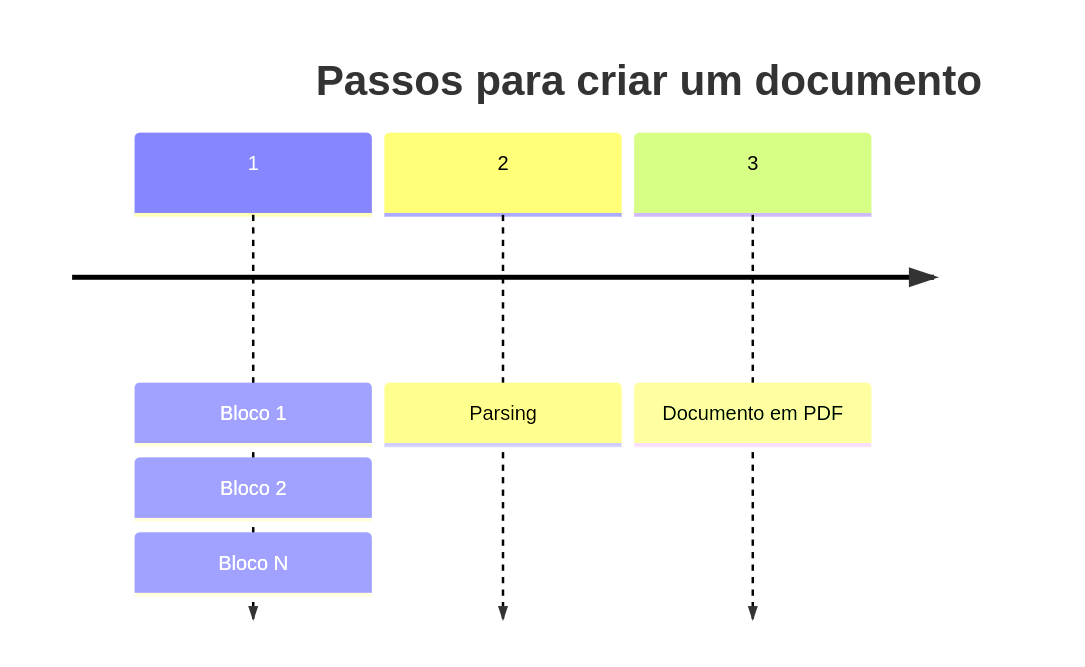
\includegraphics[width=0.8\textwidth]{./images/Passos para criar um documento.png}
    \label{fig:Passos para criar um documento} \\
    \textnormal{\fontsize{10pt}{12pt}Fonte: Autoria própria}
\end{figure}

O usuário interagirá com a aplicação escrevendo blocos que serão transformados
no documento final em
\acrshort{pdf}
. A este processo denominar-se-á Parsing. Após este, bastará
enviar o download do \acrshort{pdf}
ao usuário com todo o padrão de formatação. Os trabalhos desenvolvidos nesta plataforma
terão então duas versões: A versão de blocos, (sem formatação e interativa); e a versão
final já formatada em \acrshort{pdf}.

\section{Fluxo do documento}

\subsection{Escrita em blocos}

A escrita se dará de modo em que tudo será considerado um bloco.
A escrita em blocos consiste numa abordagem em que o texto vai sendo
escrito em seu fluxo natural, porém blocos podem ser adicionados à escrita.
Um bloco é um elemento adicionado ao fluxo de trabalho que desempenha um papel
que o diferencia dos demais blocos.
Por exemplo: Uma imagem pode ser considerada um bloco nesta abordagem, uma vez
que não é um texto mas tem o objetivo de fornecer informações visuais. O próprio corpo
do texto em si será considerado um bloco, denominado parágrafo. Um título será um bloco
textual cujo objetivo será separar sessões do texto coesas. Uma lista será um bloco para enumerar
itens e assim por diante. O documento será basicamente uma composição de diversos blocos dispostos de forma a formar
uma unidade coesa final, que será o trabalho propiamente dito.

\subsection{Bloco}

Um bloco é uma unidade lógica no documento que desempenha um papel especializado que nenhum
outro bloco o faz. Por exemplo: O bloco mais importante da
plataforma\footnote{O termo plataforma será utilizado
    de forma intercambiável e como sinônimo de aplicativo; sistema web; ou aplicativo da web}
será o de texto, (denominado bloco parágrafo), pois sem texto, não há trabalho.
Sem texto não há tão pouco comunicação que transmita informação
de caráter acadêmico-científico.

Semelhante ao bloco de texto, diversos outros blocos adjascentes
auxiliarão na construção do documento acadêmico. O bloco de imagem, por
exemplo, ajuda a exibir informações de forma ilustrativa e auxilia bastante
em exemplos que estão sendo dados em determinado contexto do texto.

A maior parte dos blocos contará com uma espécie de submenu, (em termos de aplicação),
que os permita personalizar. A personalização de blocos é importante para editar
configurações e dar autonomia ao usuário em determinar mais precisamente o papel
daquele bloco no texto. Por exemplo: Um bloco de título ajuda a separar o texto
em unidades coesas. Porém, existem diversos tipos de títulos: Existe o título, o
subtítulo, e até o subtítulo do subtítulo.

O submenu será a configuração que o usuário fará no bloco após escolhê-lo. No
caso do título, por exemplo: Após o usuário escolher este bloco, poderá configurar
o nível de título desejado. Nível este que varia do 1 ao 5, sendo 2; 3; 4 e 5
espécies de subtítulos. No caso de uma imagem, o submenu funcionará para que possa
ser definida a imagem, bem como seu título de sua descrição.

A
Figura \ref{fig:blocos-no-documento}
ilustra a composição de um trabalho com seus respectivos blocos:

\begin{figure}[H]
    \centering
    \caption{Divisão de blocos em um documento}
    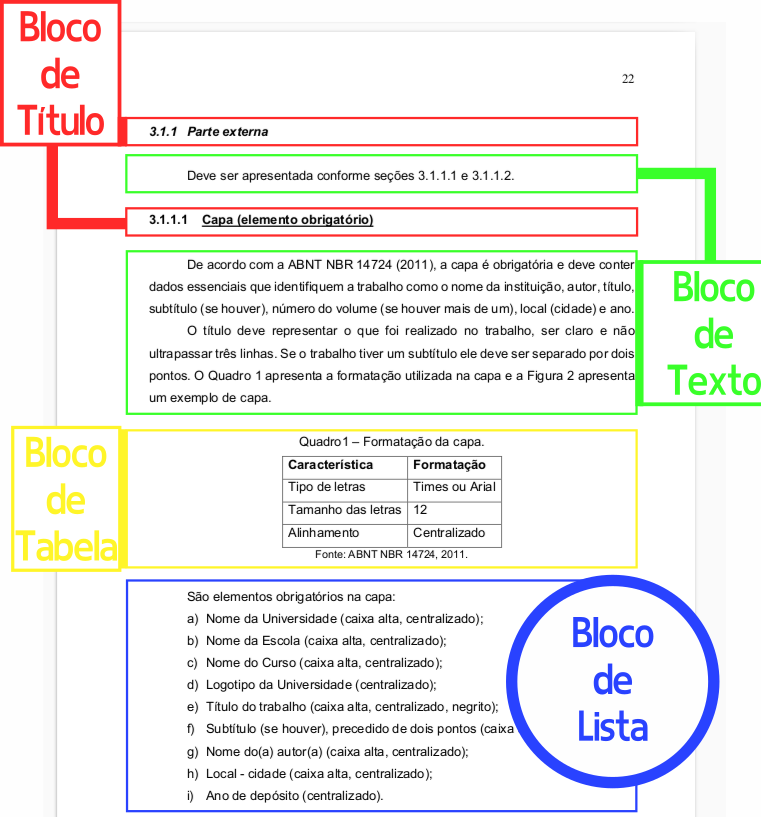
\includegraphics[width=0.8\textwidth]{./images/blocos-no-documento.png}
    \label{fig:blocos-no-documento} \\
    \textnormal{\fontsize{10pt}{12pt}Fonte: Adaptado de \cite{pucgo}}
\end{figure}

\subsection{Parsing}

O processo de Parsing é o processo que acontecerá sempre que o usuário desejar
ver o
\textit{layout}\footnote{Do inglês: Disposição, ou esboço. Esta palavra geralmente está associada ao desenho ou visual de algo.
}
da versão final de seu trabalho. Ele usa o código intermediário gerado pelos blocos para montar o
\acrshort{pdf}
final.

Este processo é, em termos simples, uma espécie de análise a ser aplicada no código gerado pelos blocos
da aplicação. A plataforma gerará um código
\acrshort{json}\footnote{Ver (sessão que trata do JSON)
}
como resultado das interações do usuário, que posteriormente
serão convertidos em código
\acrshort{latex}\footnote{Ver (sessão que trata do \acrshort{latex})
}.
Só então, finalmente será utilizado um utilitário que converterá o código \acrshort{latex}
em um documento
\acrshort{pdf}. A
Figura \ref{fig:app-json-latex-pdf} ilustra esse processo:

\begin{figure}[H]
    \centering
    \caption{Etapas do processo de Parsing}
    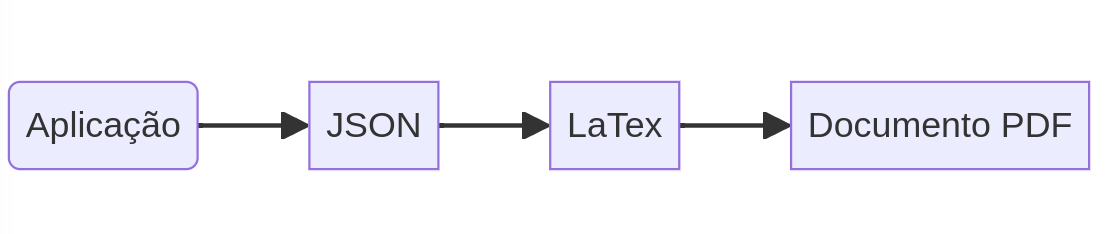
\includegraphics[width=0.9\textwidth]{./images/app-json-latex-pdf.png}
    \label{fig:app-json-latex-pdf} \\
    \textnormal{\fontsize{10pt}{12pt}Fonte: Autoria própria.}
\end{figure}

\section{Ambiente de desenvolvimento}

O ambiente de desenvolvimento é de extrema importância para que todas as ferramentas
utilizadas possam funcionar em perfeita harmonia em suas respectivas integrações e
colaborações. Muitas vezes, problemas de compatibilidade podem afetar
o funcionamento das mesmas e impedir que o programa final
seja executado corretamente, causando
\textit{bugs}\footnote{Do inglês: Inseto. Esta palavra é muito utilizada no contexto de desenvolvimento de aplicativos
para se referir a problemas que afetam o funcionamento dos mesmos
}
e outros imprevistos impeditivos tanto para a correta execução, quanto
para a exeperiência de desenvolvimento.
A
Tabela \ref{tbl:tecnologias-ambiente}                
diz respeito às ferramentas e ao ambiente onde este
\textit{software}\footnote{O software é o conjunto de instruções dadas a um computador, de modo que
    ele execute determinada tarefa. Pode-se dizer que o software é
    a parte lógica do sistema computacional.  \\  \cite{hardware-e-software}.
}
foi desenvolvido, bem como todas as suas respectivas versões:

\clearpage

\subsection{Tecnologias do ambiente de desenvolvimento}

Atender aos requisitos mínimos de
\textit{hardware}\footnote{Com hardware, compreende-se o equipamento físico de um sistema computacional.
    Suas unidades Lógicas de Processamento, memórias e unidades de armazenamento são
    hardware.  \\  \cite{hardware-e-software}.
}
e software é fundamental para garantir uma experiência de usuário satisfatória
e evitar problemas de desempenho ou compatibilidade com o aplicativo da plataforma.
A seguir
na
Tabela \ref{tbl:tecnologias-ambiente}
enumera-se o ambiente mínimo com seus respectivos
\textit{softwares}
necessários
para rodar o aplicativo da plataforma:

\begin{table}[H]
    \centering
    \caption{Tecnologias do ambiente de desenvolvimento}
    \label{tbl:tecnologias-ambiente}
    \renewcommand{\arraystretch}{1.5}
    \begin{tabular}{p{6.4000cm} p{9.6000cm}}
        \hline
        \textbf{Tipo} & \textbf{Tecnologia} \\
        \hline
        Versionador & Git 2.34.1 \\
		AbnTeX2 & 1.9.7 2018-11-24 \\
		Interpretador & NodeJs 20.10.0 \\
		Sistema Operacional & Ubuntu 20.04 \\
		Gerenciador de pacotes & Npm 10.2.3 \\
		Gerenciador de pacotes & Yarn 1.22.19 \\
		Utilitário & kpathsea version 6.3.4/dev \\
		Linguagem de Programação & TypeScript 5.3.3 \\
		Utilitário & BibTeX 0.99d (TeX Live 2022/dev/Debian) \\
		Navegador de Internet & Google Chrome 119.0.6045.199 \\
		Compilador & pdfTeX 3.141592653-2.6-1.40.22 (TeX Live 2022/dev/Debian) \\
		Utilitário & makeglossaries (Utilitário \acrshort{latex}) \\
        \hline
        \\\multicolumn{2}{c}{\fontsize{10pt}{12pt}Fonte: Autoria própria}
    \end{tabular}
\end{table}

\subsection{Tecnologias do projeto}

A seguir
na
Tabela \ref{tbl:tecnologias-projeto}
estão listadas as tecnologias exatas do projeto juntamente com
suas respectivas versões. As mesmas podem ser baixadas após o download do
repositório com qualquer gerenciador de pacotes NodeJs, tais como: npm;
yarn; pnpm e bun. Este trabalho utilizou o yarn:

\begin{table}[H]
    \centering
    \caption{Tecnologias do projeto}
    \label{tbl:tecnologias-projeto}
    \renewcommand{\arraystretch}{1.5}
    \begin{tabular}{p{3.2000cm} p{4.8000cm}}
        \hline
        \textbf{Nome} & \textbf{Versão} \\
        \hline
        antd & \textasciicircum 5.15.0 \\
		next & \textasciicircum 14.1.1 \\
		react & \textasciicircum 18.2.0 \\
		node-latex & \textasciicircum 3.1.0 \\
		cheerio & \textasciicircum 1.0.0-rc.12 \\
		@editorjs/list & \textasciicircum 1.9.0 \\
		@editorjs/header & \textasciicircum 2.8.1 \\
		@emotion/react & \textasciicircum 11.11.4 \\
		@emotion/styled & \textasciicircum 11.11.0 \\
		@editorjs/editorjs & 2.29.1 \\
        \hline
        \\\multicolumn{2}{c}{\fontsize{10pt}{12pt}Fonte: Autoria própria}
    \end{tabular}
\end{table}

\subsection{Versionador, (Versão do projeto)}

Este trabalho utiliza o Git para controlar suas respectivas versões e
evolução. Como o código é dinâmico e está sempre evoluindo,
os exemplos fornecidos neste documento estão registrados numa determinada
versão específica afim de que não se perca o exemplo dado com código que
poderá estar diferente dependendo da data em que o trabalho for lido.

Todos os exemplos em código fornecidos, bem como a correspodência de linhas
estão presentes nos detalhes da versão de
commit\footnote{Um commit, (nos termos do git), é como salvar o projeto, guardando uma versão do código naquele momento específico.
    O commit pode ser comparado a uma foto do projeto, capturando o estado atual e todas as mudanças feitas desde o último commit.
}
abaixo:

\begin{GitVersionCode}
commit c0cab19296c46355d4bee5cc3e164616ed73fe49
Author: Higor Ferreira <hfashigor@hotmail.com>
Date:   Sun Jun 9 11:03:02 2024 -0300

    updateDocs: README
\end{GitVersionCode}

\chapter{Fundamentação teórica}

A plataforma será construída sob alguns pilares fundamentais indispensáveis
a seu funcionamento. São estes pilares que garantirão o sucesso e o correto
funcionamento da aplicação, afim de que todo o objetivo discutido até o
presente momento seja atingido.

A
Figura \ref{fig:pilares-da-plataforma}
mostra em forma de mapa mental todos os principais pilares sobre os quais
o aplicativo será contruído. Estes pilares são formados por diversas
tecnologias, bibliotecas,
\textit{frameworks}\footnote{Uma framework é como um kit de ferramentas pré-pronto que fornece uma gama
    de funcionalidades pré-construídas e testadas afim de facilitar o processo
    de desenvolvimento. \cite{amazon-framework}
}
e conceitos que deverão trabalhar de forma integrada.

\begin{figure}[H]
    \centering
    \caption{Pilares da plataforma, (mapa mental)}
    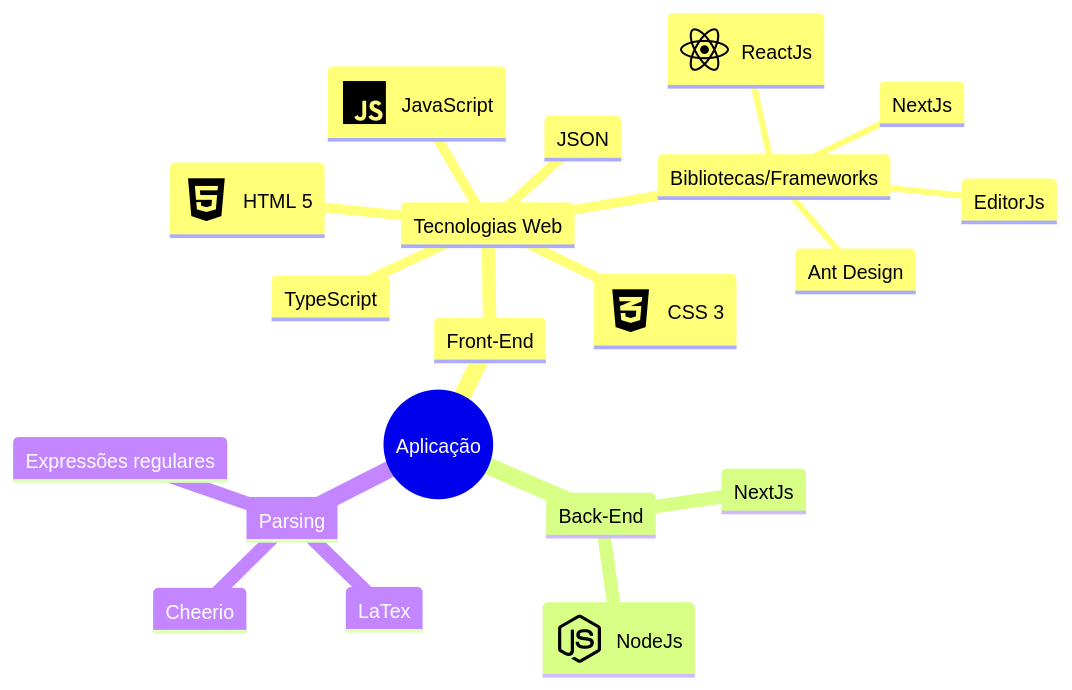
\includegraphics[width=0.9\textwidth]{./images/pilares-da-plataforma.png}
    \label{fig:pilares-da-plataforma} \\
    \textnormal{\fontsize{10pt}{12pt}Fonte: Autoria própria.}
\end{figure}

Estes pilares estão subdivididos em três grandes subcategorias, a saber: Front-End;
Back-End e Parsing. Cada qual com seus respectivos conceitos e tecnologias.

\section{Do Front-End}

O
\textit{Front-End}
é, basicamente, a "linha de frente". É a parte da aplicação que interagirá
diretamente com o usuário. Ao profissional que codifica e desenvolve esta parte do
projeto, denomina-se Desenvolvedor Front-End. A interface do usuário, que é
onde o mesmo realiza suas interações com o sistema, normalmente é desenhada por
um
\textit{designer}\footnote{Profissional que atua com design.
}
, ficando a cardo do desenvolvedor o papel de adaptar o
\textit{design}\footnote{Do inglês: Desenho.
}
ao código afim de obter os efeitos desejados.
\cite{totvs-front-end}

\subsection{Tecnologias Web}

As tecnologias
\acrshort{web}
desempenham um papel crucial na criação de experiências
digitais interativas, permitindo que os usuários se envolvam com o conteúdo de maneira mais
dinâmica e significativa. A incorporação da
\textit{Internet}\footnote{Rede mundial de computadores, \cite{marco-civil-art-2}.
}
na vida diária resultou em mudanças
significativas, marcada por um ritmo de evolução e aprimoramento sem precedentes, além da
distribuição de conteúdo em massa. Juntamente com essas mudanças, surgiram novas
tecnologias, variando de
\textit{softwares}
a
\textit{hardwares},
aprimorando a experiência de navegação na
\acrshort{web}
\cite{molgado}.

A Internet, que teve origem nos Estados Unidos em 1969, foi inicialmente utilizada
por universidades, governos e instituições financeiras antes de se expandir globalmente. No
início, a internet era uma via de mão única onde os usuários consumiam informações e se
comunicavam de maneira privada. A evolução começou com a introdução de sistemas de
busca avançados, destacando-se o lançamento do Google em 1998, que democratizou o
acesso à informação.
\cite{vitoriano}.

A grande reviravolta na internet aconteceu em 1999, com o surgimento do
\textit{Blogger},
marcando o início da
Web
2.0, onde a comunicação tornou-se bidirecional. Os usuários
passaram a gerar conteúdo e se relacionar publicamente com marcas, empresas e pessoas por
meio de comentários, além de consumir informação. A evolução da tecnologia móvel, em
conjunto com o surgimento de redes sociais como
\textit{Fotolog},
\textit{MySpace},
\textit{Orkut},
\textit{Facebook},
\textit{YouTube}
e
\textit{Twitter},
ampliou o conceito de Web 2.0, permitindo o compartilhamento de fotos,
vídeos e textos em uma escala maior.
\cite{vitoriano}.

A forma como se interage com a internet também evoluiu ao longo do tempo.
Passou-se de sites estáticos para interativos e animados, chegando até aos sites totalmente
responsivos\footnote{A responsividade é a capacidade de uma página da
    \acrshort{web}
    em se adaptar a diferentes dispositivos e tamanhos de tela.
    \cite{responsivo}
}
e adaptáveis de hoje. Isso foi possível devido ao desenvolvimento de novos
gadgets e ao surgimento de novas linguagens de programação. Atualmente, a Web Moderna é
composta por várias técnicas, metodologias, linguagens e ferramentas que permitem o
desenvolvimento de aplicações conectadas e interativas, oferecendo diversas formas de
interação com interfaces digitais.
\cite{vitoriano}.

\subsubsection{\underline{Linguagem de Marcação de Hipertexto, HTML}}

A Linguagem de Marcação de Hipertexto, do inglês: \textit{HyperText Markup Language}
(\acrshort{html})
foi criada por Tim Berners-Lee enquanto trabalhava na Organização Europeia para a
Pesquisa Nuclear
(\acrshort{cern}),
o laboratório de física de partículas na Suíça, no final dos anos
1980 e início dos anos 1990. O objetivo era criar uma maneira de compartilhar documentos e
informações em um ambiente de rede. A primeira versão do
\acrshort{html}
tinha apenas 18 elementos
de marcação, permitindo a formatação básica de texto e a inclusão de
\textit{links}\footnote{Do inglês: Ligação. Também chamado de hiperlink, é uma referência a um
    documento eletrônico que, quando clicado, leva o usuário para outro recurso
    ou documento.
},
imagens e listas.
\cite{w3c}.

O
\acrshort{html}
rapidamente ganhou popularidade e passou por várias iterações, cada uma
adicionando novos elementos e funcionalidades. O
\acrshort{html}4,
lançado em 1997, trouxe uma
série de melhorias, incluindo mais controle sobre a aparência das páginas web, a introdução
de folhas de estilo em cascata
(\acrshort{html})
e melhor suporte a
\textit{scripts}\footnote{Do inglês: Roteiro. Aqui usado no sentido de código fonte, que nada mais são
    do que um conjunto de instruções que o computador seguirá de modo interpretativo.
}.
\cite{w3c}.

Finalmente, o
\acrshort{html}5,
lançado oficialmente em 2014 pelo
\textit{World Wide Web Consortium}
(\acrshort{w3c}), trouxe uma série de novas funcionalidades, incluindo suporte nativo para
vídeo e áudio; novos elementos semânticos; gráficos e animações; geolocalização;
armazenamento local e muito mais.
\cite{w3c}.

\subsubsection{\underline{Funcionamento do HTML}}

O
\acrshort{html}
funciona como uma linguagem de marcação, o que significa que ele usa
\textit{"tags"}\footnote{Do inglês: Marcação.
}
para definir diferentes partes de um documento. Essas tags informam ao navegador
como exibir o conteúdo da página. Por exemplo, a tag
<p>
é usada para definir um parágrafo,
enquanto a tag
<h1>
é usada para definir um cabeçalho de primeiro nível.
\cite{w3c}.

As páginas
\acrshort{html}
são estruturadas usando uma combinação de elementos de bloco,
(que formam a estrutura principal da página), e elementos
\textit{inline}\footnote{Do inglês: Dentro da Linha. São elementos que podem ser escritos sem quebra de linha.
},
(que formatam o conteúdo
dentro desses blocos). Os elementos são aninhados dentro de outros elementos para criar a
estrutura hierárquica da página.
\cite{w3c}.

\subsubsection{\underline{HTML versão 5}}

Com o
\acrshort{html}5,
os desenvolvedores podem criar jogos online, reproduzir vídeos e
áudios diretamente no navegador, tudo isso sem a necessidade de instalação de plugins
externos. Isso resultou em uma melhor experiência geral do usuário, com carregamento mais
rápido e maior compatibilidade entre os navegadores.
\cite{w3c}.

Além disso, o
\acrshort{html}5
também trouxe recursos avançados de armazenamento local,
como o
\textit{\acrshort{web} Storage}\footnote{O termo
    \acrshort{web} Storage pode ser entendido, em tradução
    livre, como: Armazém da \acrshort{web}
}
e o
\textit{IndexedDB}\footnote{Termo abreviado de "Indexed DataBase", (Base de Dados Indexada).
}.
Esses recursos permitem que os sites armazenem dados
localmente no navegador do usuário, possibilitando a criação de aplicativos web
\textit{offline}
e
sincronização de dados em tempo real.
\cite{w3c}.

Outra contribuição importante do
\acrshort{html}5
é o suporte a tecnologias de
geolocalização e acesso aos recursos do dispositivo. Isso permite que os desenvolvedores
acessem informações de localização do usuário, câmera, microfone e acelerômetro, abrindo
possibilidades para o desenvolvimento de aplicativos web que utilizam esses recursos de
forma integrada.
\cite{w3c}.

Ao longo de sua história, o
\acrshort{html}
tem evoluído constantemente para acompanhar as
demandas e os avanços tecnológicos da web. O
\acrshort{html}5
é um marco significativo nessa
evolução, trazendo recursos semânticos, multimídia e interativos para a criação de páginas da
web modernas.
\cite{w3c}.

\subsubsection{\underline{Folhas de Estilo em Cascata, (CSS)}}

Folhas de Estilo em Cascata, ou \textit{Cascading Style Sheets}
(\acrshort{css}),
em tradução livre
para o português, é uma linguagem de estilo altamente eficaz e amplamente utilizada. Sua
principal função é definir a apresentação de documentos escritos em
\acrshort{html}
ou
\acrshort{xml}.
Isso
inclui uma série de linguagens baseadas em
\acrshort{xml},
como
\acrshort{svg},
\acrshort{mathml}
e
\acrshort{xhtml}.
O
\acrshort{css}
é
responsável por descrever a forma como os elementos são apresentados em diferentes mídias,
seja na tela do computador, em papel impresso, por meio de dispositivos de fala ou em outras
formas de mídia.
\cite{mdn-css}.

Considerado uma das principais linguagens da
Open\footnote{Do inglês: Aberto. Neste contexto, refere-se ao padrão "Aberto"~ da
    \acrshort{web}
}
\acrshort{web},
o
\acrshort{css}
tem uma grande
importância na padronização dos navegadores
\acrshort{web}.
Essa padronização é feita de acordo com
as especificações estabelecidas pela
\acrshort{w3c},
a organização que lidera a
\acrshort{web}
mundial. O
desenvolvimento do
\acrshort{css}
é feito em níveis distintos: o
\acrshort{css}1,
que hoje é considerado
obsoleto; o
\acrshort{css}2.1,
que atualmente é uma recomendação; e o
\acrshort{css}3,
que está sendo dividido
em pequenos módulos e caminha para a sua padronização.
\cite{mdn-css}.

\subsubsection{\underline{JavaScript}}

JavaScript é uma linguagem de programação notavelmente versátil que, apesar de ser
comumente conhecida pela sua utilização em páginas
\acrshort{web}, vai muito além disso.
Frequentemente abreviada para 
\acrshort{js}, essa linguagem é leve, interpretada e orientada a objetos
com funções de primeira classe. Graças à sua flexibilidade, o JavaScript se expandiu para uma
variedade de ambientes que não são navegadores, incluindo
Node.Js\footnote{Ver sessão que trata do Node.Js
},
Apache CouchDB\footnote{Base de dados que utiliza o JSON nativamente. Veja mais em:  \\ https://couchdb.apache.org/\#about
}
e
Adobe Acrobat\footnote{Software que lê e converte arquivos em formato
    \acrshort{pdf}. Veja mais em:  \\ https://www.adobe.com/br/acrobat.html
},
demonstrando sua adaptabilidade e eficácia em diversos contextos.
\cite{mdn-js}.

Com sua estrutura baseada em protótipos, o JavaSript é uma linguagem dinâmica que
suporta múltiplos paradigmas de programação. Isso significa que, além de ser orientada a
objetos, ela também suporta estilos de programação imperativos e declarativos, como a
programação funcional. Essa capacidade de suportar diferentes estilos de programação torna o
JavaScript uma ferramenta poderosa e flexível para os desenvolvedores.
\cite{mdn-js}.

O padrão para JavaScript é o
\acrshort{ecma}Script.
Desde 2012, todos os navegadores
modernos oferecem suporte completo ao
\acrshort{ecma}Script 5.1. Mesmo os navegadores mais
antigos fornecem suporte, pelo menos, ao
\acrshort{ecma}Script 3. A sexta versão do
\acrshort{ecma}Script,
oficialmente chamada de
\acrshort{ecma}Script 2015 e inicialmente conhecida como
\acrshort{ecma}Script 6
ou ES6, foi publicada pela \acrshort{ecma} International
em 17 de junho de 2015. Desde então, as
especificações do
\acrshort{ecma}Script são lançadas anualmente, demonstrando o desenvolvimento
contínuo e o avanço dessa linguagem padrão.
\cite{mdn-js}.

\subsubsection{\underline{TypeScript}}

O TypeScript, as vezes abreviado como
\acrshort{ts}, é uma linguagem fortemente
tipada construída em cima do JavaScript,
\cite{ts-page}.
Typescript traz uma sintaxe adicional para o JavaScript de modo
que o mesmo possa suportar checagem de tipos estática.
Sem o \acrshort{ts},
fica difícil saber com quais tipos de dados estar-se a trabalhar
durante o processo de desenvolvimento, pois o JavaScript é uma
linguagem fracamente tipada. Os parâmetros das funções e variáveis
não possuem nenhuma informação, forçando os desenvolvedores
a recorrerem a todo momento à documentação ou intuir sobre
as tipagens.
Typescript resolve esse problema, permitindo tipar o código
de modo que erros possam ser reportados quando a tipagem estiver
incorreta, por exemplo: ao tentar-se passar uma
string\footnote{Do inglês: Corda, barbante ou fio. No contexto de programação,
    é usado como termo para cadeira de caracteres. O caractere é, na
    maioria das linguagens de programação, um tipo de dado. E textos
    são formados por estas cadeias denominadas strings,
}
para uma função que espera um número, TypeScript lançará um erro.
O JavaScript, por outro lado, permitirá a execução deste código
podendo gerar erros de tempo de execução.
\cite{ts-w3}.

O TypeScript possui um compilador, que nada mais é do que um
transpilador. Este transpilador é responsável por transformar o
código
\acrshort{ts} em
\acrshort{js}.
Desta forma, o código JavaScript resultante da
transpilação pode ser rodado em praticamente qualquer
navegador ou ambiente que suporte o JavaScript.

\subsubsection{\underline{JavaScript Object Notation, JSON}}

\textit{JavaScript Object Notation}, (Notação de Objeto JavaScript),
popularmente chamado de \acrshort{json}. É uma sintaxe para a serialização de
objetos do javascript. Com objetos do javascript, compreende-se seus tipos
de dados e valores, como: objetos; matrizes; números; strings; booleanos;
\textit{null}\footnote{Do inglês: Nulo. Neste contexto é um valor especial do JavaScript para
    representar a nulidade de um objeto/variável.
}
e
\textit{undefined}\footnote{Do inglês: Indefinido. Neste contexto é um tipo de dado do JavaScript
    para variáveis indefinidas.
}.
Apesar de baseado na sintaxe do JavaScript, distingue-se desta
no sentido da forma de escrita. A serialização é o processo
de converter dados estruturados, (ou objetos), em um formato que pode
facilmente ser armazenado e transmitido pela rede. O \acrshort{json}
basicamente converte os objetos JavaScript em strings. Uma caracteristica deste,
é que \acrshort{json} é legível tanto por humanos, quanto por máquinas,
(na maioria dos casos).
\cite{mdn-json}.

A
Tabela \ref{tbl:json-descs}
mostra as principais
diferenças entre o JavaScript e o JSON.

\begin{table}[H]
    \centering
    \caption{Diferenças entre o JavaScript e o JSON}
    \label{tbl:json-descs}
    \renewcommand{\arraystretch}{1.5}
    \begin{tabular}{p{5.6000cm} p{10.4000cm}}
        \hline
        \textbf{Tipos e valores JavaScript} & \textbf{Diferença para o JSON} \\
        \hline
        Objetos e Arrays & Os nomes das propriedades devem ser strings com aspas duplas; as vírgulas à direita são proibidas. \\
		Números & Zeros à esquerda são proibidos; um ponto decimal deve ser seguido por pelo menos um dígito. \\
		Strings & Apenas um conjunto limitado de caracteres pode ser escapado; certos caracteres de controle são proibidos; o separador de linha Unicode (U+2028) e o separador de parágrafo (U+2029) são permitidos; strings devem ter aspas duplas.
             \\
        \hline
        \\\multicolumn{2}{c}{\fontsize{10pt}{12pt}Fonte: \cite{mdn-json}.}
    \end{tabular}
\end{table}

\subsection{Bibliotecas e Frameworks}

\subsubsection{\underline{ReactJs}}

\begin{figure}[H]
    \centering
    \caption{Logotipo do React}
    
\includegraphics[width=0.8\textwidth]{./images/react-logotipo.png}
    \label{fig:react-logotipo} \\
    \textnormal{\fontsize{10pt}{12pt}Fonte: React Dev, disponível em: https://react.dev/}
\end{figure}

"Biblioteca para interfaces de usuário \acrshort{web} e nativas".
O React é uma biblioteca de JavaScript criada pelo Facebook para solucionar
desafios de manutenção e escalabilidade em suas aplicações. No início de 2011, a equipe de
desenvolvedores do Facebook enfrentava dificuldades em lidar com o crescimento da
aplicação de anúncios, que estava se tornando cada vez mais complexa e difícil de ser
mantida. O aumento no número de membros da equipe e de funcionalidades estava afetando
negativamente os processos da empresa. Com tantas atualizações em cascata, a aplicação
estava se tornando lenta e difícil de ser atualizada sem falhas.
\cite{morais-react}.

Para resolver esses problemas, Jordan Walke, engenheiro do Facebook, propôs uma
solução inovadora. Ele sugeriu levar o 
XHP,
uma versão do
\acrshort{php},
para o navegador usando
JavaScript. O 
XHP
era uma tecnologia desenvolvida para minimizar ataques de Cross-Site
Scripting
(\acrshort{xss})
em aplicações
\acrshort{web}
dinâmicas. No entanto, ele não era capaz de lidar com o
grande número de requisições necessárias para esse tipo de aplicação. Com o apoio de sua
equipe de gerenciamento, Jordan Walke conduziu um experimento de seis meses para
explorar essa ideia. O resultado desse experimento foi o surgimento do ReactJS.
\cite{morais-react}.

O ReactJS revolucionou o desenvolvimento de interfaces de usuário ao introduzir o
conceito de componentes reutilizáveis e a abordagem de renderização virtual. Com a
utilização de componentes, os desenvolvedores podiam criar e reutilizar peças de interface
independentes e isoladas, o que simplificava o desenvolvimento e manutenção do código.
Além disso, a renderização virtual permitia atualizações de interface eficientes, otimizando o
desempenho da aplicação. O ReactJS foi lançado como um software de código aberto em
2013, permitindo que desenvolvedores de todo o mundo o utilizassem em seus projetos.
\cite{morais-react}.

Desde então, o React ganhou uma imensa popularidade e se tornou uma das
principais ferramentas para o desenvolvimento de interfaces de usuário em aplicações web.
Sua abordagem declarativa, que permite descrever como a interface deve ser exibida com
base no estado da aplicação, simplifica a construção de interfaces complexas. Além disso, a
capacidade de reutilização de componentes economiza tempo e esforço durante o
desenvolvimento. O React também influenciou o desenvolvimento do React Native, uma
versão da biblioteca voltada para a criação de aplicativos móveis multiplataforma. Com a
ajuda de uma grande comunidade de desenvolvedores e empresas, o ecossistema do React
continua a evoluir e fornecer soluções inovadoras para o desenvolvimento de interfaces de
usuário modernas e eficientes.
\cite{morais-react}.

O React teve seus primeiros sinais em 2010, quando o Facebook introduziu o XHP
na sua stack de
\acrshort{php},
permitindo a criação de componentes compostos. Em 2011, Jordan
Walke criou o FaxJS, protótipo inicial do React, que foi desenvolvido para resolver os
desafios de suporte aos anúncios do Facebook. Em 2012, o Instagram foi adquirido pelo
Facebook e expressou interesse em adotar o React. Isso levou o Facebook a dissociar o React
da empresa e torná-lo open source. Em 2013, ocorreu o lançamento oficial do React, mas
inicialmente enfrentou resistência da comunidade de desenvolvedores. No entanto, uma "turnê
do React"~ foi realizada para conquistar os não adeptos.
\cite{morais-react}.

No ano seguinte, o React começou a ganhar reputação e confiança. O
\textit{React Developer Tools}\footnote{Ferramentas de Desenvolvimento React
}
e o
\textit{React Hot Reloader}\footnote{Carregamento e recarregamento ultra rápido React
}
foram lançados, trazendo melhorias no
desenvolvimento e na experiência do usuário. Em 2015, o React se estabeleceu como uma
tecnologia estável, com empresas como Netflix e Airbnb adotando-o. O Redux, responsável
pelo gerenciamento de estado, foi lançado, e o React Native expandiu-se para o
desenvolvimento de aplicativos móveis para Android.
\cite{morais-react}.

Atualmente, o React continua evoluindo, com o lançamento de novas
funcionalidades e recursos para melhorar o desenvolvimento de aplicações. Iniciativas de
\acrshort{ssr}
\textit{(Server Side Rendering)}\footnote{Do inglês: Rederização do Lado do Servidor
}, e o foco em componentes funcionais são algumas das áreas de
desenvolvimento. O React permanece como uma biblioteca consolidada no mercado de
Front-End, sendo amplamente adotado por grandes empresas em todo o mundo.
\cite{morais-react}.

\subsubsubsection{JavaScript XML}

O JavaScript XML, (\acrshort{jsx}),
é uma extensão de sintaxe para o JavaScript que permite escrever
código de marcação, (como o \acrshort{html}),
dentro do JavaScript. Os componentes React nada mais são do que
funções ou classes chamadas a partir do código
\acrshort{js}
que atualizam o
\acrshort{html}
através da
\textit{Document Object Model}\footnote{Do inglês: Modelo de Documento de Objeto. O
    \acrshort{dom}
    é utilizado pelo JavaScript para manipular o documento
    \acrshort{html}
    exibido em tela.
    \cite{alura-dom}
 },
(\acrshort{dom}).
O
\acrshort{jsx}
facilita esse trabalho. Pois ao invés de chamar
funcões ou instanciar classes no código JavaScript,
pode-se escrever a marcação diretamente no mesmo,
como se o 
\acrshort{html}
estivesse dentro do
\acrshort{js}.
\cite{react-jsx}.

A
Figura \ref{fig:exemplo-jsx}
mostra um exemplo de código em
\acrshort{jsx}.
É exportada uma função denominada \textit{TodoList},
que nada mais é do que um componente React.
Esta função retorna um determinado valor, que é
o código
\acrshort{jsx}
propriamente dito. Este código será renderizado
no lugar onde esta função for chamada.

\begin{figure}[H]
    \centering
    \caption{Exemplo de código JSX}
    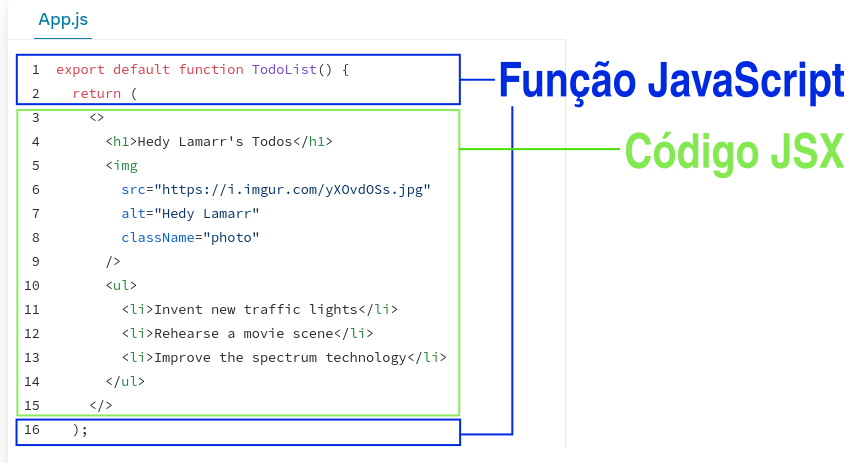
\includegraphics[width=0.9\textwidth]{./images/exemplo-jsx.png}
    \label{fig:exemplo-jsx} \\
    \textnormal{\fontsize{10pt}{12pt}Fonte: Adaptado de: ReactJs. Disponível em: <https://pt-br.react.dev/learn/writing-markup-with-jsx>}
\end{figure}

\subsubsection{\underline{NextJs}}

\begin{figure}[H]
    \centering
    \caption{Logotipo do NextJs}
    
\includegraphics[width=1.0\textwidth]{./images/nextjs-logotipo.png}
    \label{fig:nextjs-logotipo} \\
    \textnormal{\fontsize{10pt}{12pt}Fonte: Next.Js, disponível em: https://nextjs-template.vercel.app/}
\end{figure}

O NextJs é uma framework em ReactJs voltada à construção de aplicações
\acrshort{web}
tando na parte do Front-End quanto no Back-End.
Com NextJs, utiliza-se os componentes em React para construir as interfaces
de usuário, com o NextJs provendo recursos adicionais e otimizações.
\cite{nexjs-docs}.

NextJs também se encarrega de todas as configurações necessárias do React, como o processo
de
enpacotamento\footnote{Em inglês: Bundling. Um Bundle para a \acrshort{web},
    por exemplo, junta todos os códigos e recursos em um pacote otimizado
    para ser distribuído.
},
compilação e etc...
Permitindo ao desenvolvedor apenas focar no desenvolvimento da aplicação em si.
\cite{nexjs-docs}.

Devido à natureza desta framework, O NextJs é um pilar que aparece
tanto no Back-End quanto no Front-End. Estas duas frentes serão abordadas
com a utilização desta ferramenta, aproveitando ao máximo os recursos fornecidos
pela mesma. Os principais recursos oferecidos pelo NextJs são:

\begin{itemize}
        
	\item Roteamento: O NextJs provê um roteamento, (que é basicamente a navegação por páginas
                    dentro do app), baseado no sistema de arquivos do Sistema Operacional. Os arquivos
                    em pastas do projeto são mapeados para links, que fornecem os componentes de servidor
                    com suporte a
                    layouts\footnote{Layouts são como templates que são comuns às páginas roteadas. Ajudam no processo
                        de reaproveitamento de componentes pois eles podem ser extendidos às páginas,
                        que herdam características destes layouts.
                    },
                    rotas aninhadas, estados de carregamento, manipulação de erros,
                    entre outros...
                
	\item Renderização: NextJs fornece renderização do lado do cliente e do lado do servidor com
                    componentes de cliente, e componentes de servidor.
                
	\item Busca de dados: Há um processo de busca de dados simplificado com o uso de
                    \textit{async/await}\footnote{Recurso do JavaScript para lidar com a execuçao de código assíncrono.
                    }
                    nos componentes de servidor, além de uma
                    \acrshort{api}\footnote{Do inglês: Interface de Programação de Aplicações. É uma forma na qual
                        dois ou mais aplicativos ou componentes de de computador se comunicam
                        entre si. É uma interface de software que oferece um serviço para outras
                        partes do mesmo ou de outros softwares.
                        \cite{api-reddy}.
                    }
                    expandida para a memorização das
                    requisições,
                    \textit{caching}\footnote{O processo de caching é o ato de armazenar informações que são acessadas
                        frequentemente de maneira que seu acesso se torne mais rápido. Neste contexto,
                        o resultado de uma requisição pode ser armazenado em cache para que não
                        seja necessário consultar o servidor novamente quando a mesma informação
                        for requisitada.
                    }
                    de dados e revalidação.
                
	\item Estilização: Suporte para os métodos preferidos de estilização. Com inclusão
                    de: Módulos \acrshort{css}, \textit{Tailwind} \acrshort{css},
                    e \acrshort{css}-in-\acrshort{js}.
                
	\item Otimizações: Otimizações de scripts, imagens e fontes são também fornecidos para aprimorar
                    o núcleo do aplicativo e a experiência de usuário.
                
	\item TypeScript: Suporte total ao TypeScript, com uma melhor checagem de tipos e compilação eficiente.
                
    
\end{itemize}

\cite{nexjs-docs}.
            

\subsubsection{\underline{EditorJs}}

\begin{figure}[H]
    \centering
    \caption{Logotipo do EditorJs}
    
\includegraphics[width=0.8\textwidth]{./images/editorjs-logotipo.png}
    \label{fig:editorjs-logotipo} \\
    \textnormal{\fontsize{10pt}{12pt}Fonte: Editor.Js, disponível em: https://editorjs.io/}
\end{figure}

"Editor livre em blocos com saída universal em JSON".
O EditorJs é um rico editor de texto em blocos que oferece uma experiência de
edição intuitiva e versátil. Tudo o que é feito no EditorJs no fim é transformado
em um arquivo \acrshort{json} ao invés de um documento de marcação
em \acrshort{html}.
Essa abordagem deixa o processo mais simples para os desenvolvedores no
sentido de projetarem suas próprias integrações. Assim, o EditorJs pode ser
aplicado a diversas plataformas.
\cite{editorjs}.

São recursos do EditorJs:

\begin{itemize}
        
	\item Dados de saída limpos
	\item \acrshort{api} baseada em plugins
	\item Código aberto
    
\end{itemize}

O espaço de trabalho do EditorJs consiste em blocos separados, como:
Parágrafos; títulos; listas; etc... Cada um deles independentes entre si,
com muitos outros recursos como: Copiar e colar; seleção de vários blocos;
e entre outros que funcionam de forma familiar a outras ferramentas.
\cite{editorjs}.

O conceito chave do EditorJS é sua \acrshort{api}, na qual
todas as unides funcionais do editor são providas através de plugins externos que fazem
uso da mesma. Assim, o núcleo do EditorJs fica sendo mais abstrato e poderoso, de
modo que o desenvolvedor possa implementar diversos desafios com a criação
de seus próprios plugins.
\cite{editorjs}.

\subsubsection{\underline{AntDesign}}

\begin{figure}[H]
    \centering
    \caption{AntDesign}
    
\includegraphics[width=0.8\textwidth]{./images/antdesign-pagina-inicial.png}
    \label{fig:antdesign-pagina-inicial} \\
    \textnormal{\fontsize{10pt}{12pt}Fonte: AntDesign, Disponível em: <https://ant.design>.}
\end{figure}

"Ajudando designers e desenvolvedores a construir belos produtos de forma flexível, trabalhando com alegria.".
O AntDesign é uma biblioteca de
\acrshort{ui},
\textit{User Interface}\footnote{Do inglês: Interface de Usuário
}.
Esta biblioteca é uma grande auxiliadora na hora de produzir aplicativos
com um design agradável sem que o desenvolvedor gaste muito tempo
estilizando os componentes da aplicação.

Totalmente integrado ao ReactJs, o AntDesign já traz consigo uma vasta
gama de componentes reutilizáveis que podem ser "encaixados"~ à
construção das telas do app.
O AntDesign não impacta somente a
\acrshort{ui},
mas também a
\textit{User Experience}\footnote{Do inglês: Experiância de Usuário
},
\acrshort{ux}, uma vez que seus componentes são construídos
em cima do React. Deixando-os altamente reativos e já com seus
devidos comportamentos padrão. Ficado a cargo do desenvolvedor
apenas personalizar o que se deseja fazer.
A
Figura \ref{fig:componente-ant-ex}
mostra um exemplo de implementação de um componente em AntDesign.

\begin{figure}[H]
    \centering
    \caption{Exemplo de componente em AntDesign}
    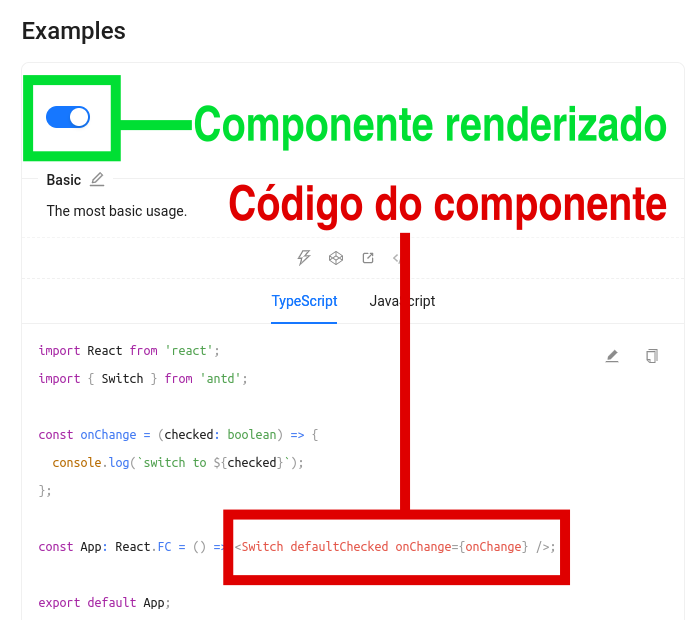
\includegraphics[width=0.9\textwidth]{./images/componente-ant-ex.png}
    \label{fig:componente-ant-ex} \\
    \textnormal{\fontsize{10pt}{12pt}Fonte: Adaptado de: AndDesign. Disponível em: <https://ant.design/components/switch>}
\end{figure}

Nota-se que com apenas uma linha tem-se um componente completo com
um visual totalmente moderno. Algo que com apenas
\acrshort{html},
\acrshort{css}
e
\acrshort{js},
gastaria algumas dezenas de linhas de código.
Tanto ReactJs quanto AntDesign significam economia
em termos de tempo, código e simplicidade de projeto.

\section{Do Back-End}

Back-end se relaciona com o que está nos bastidores das aplicações desenvolvidas na programação. Ou seja, tudo que dá estrutura e apoio às ações do usuário da máquina é chamado de back-end. Quando se acessa um site, por exemplo, por trás de toda sua apresentação amigável esteticamente, há uma comunicação das informações trocadas entre banco de dados e navegador. Portanto, atrás da interface gráfica do realizador, o back-end está sempre agindo.
\cite{totvs-back-end}.

\subsection{NodeJs}

\begin{figure}[H]
    \centering
    \caption{Logotipo do NodeJs}
    
\includegraphics[width=0.7\textwidth]{./images/logotipo-nodejs.png}
    \label{fig:logotipo-nodejs} \\
    \textnormal{\fontsize{10pt}{12pt}Fonte: Adaptado de: NodeJs. Disponível em: <https://nodejs.org/en>}
\end{figure}

"Rode JavaScript em todo lugar".
O NodeJs é um ambiente de
\textit{runtime}\footnote{Do inglês: Tempo de execução. Um runtime é basicamente um interpretador
    capaz de executar um script.
}
que permite ao desenvolvedor criar servidores, aplicativos
\acrshort{web},
ferramentas e linha de comando, entre outros...
É a principal tecnologia deste projeto e o que permitirá
a execução de todas as outras na sequência.

Antes do NodeJs, o JavaScript era uma linguagem que
rodava puramente em
\textit{Browsers}\footnote{Do inglês: Navegadores. Aqui usado no sentido de
    navegador da \acrshort{web}, ou seja,
    o aplicativo no qual acessa-se páginas na internet.
}
como uma forma de adicionar interações às páginas da internet.
Com o NodeJs, o JavaScript passou do ambiente dos Browsers
ao ambiente dos Sistemas Operacionais. Abstraindo
\acrshort{api}s
dos mesmos. Hoje, com NojeJs, por exemplo, pode-se
acessar a
\acrshort{api}
do sistema de arquivos do Sistema Operacional.
Algo que há um tempo atrás só se fazia com
linguagens de baixo nível como o C++.

A plataforma desenvolvida neste trabalho será
um servidor que distribuirá o Sistema
\acrshort{web}
que é a plataforma em si. O NextJs,
tecnologia escolhida para este fim,
é um servidor capaz de processar uma parte
das interfaces do sistema estaticamente, e
entregá-las ao cliente juntamente com os scripts
de suas partes dinâmicas. Desta forma,
ganha-se segurança no processamento back-end
ao mesmo tempo que não perde-se em termos de
interatividade com o usuário.
Há também diversos ganhos de performance e simplificação
de código, uma vez que back-end e front-end
serão concentrados no mesmo lugar, não precisando
separá-los em projetos diferentes.

\section{O processo de Parsing}

O processo de Parsing é uma das partes mais vitais deste projeto.
Sem ele, não é possível obter o documento final formatado de acordo
com as normas postas da
\acrshort{abnt}
e da
\acrshort{pucgo}.
Pode-se dizer que o Parsing é o código núcleo da aplicação, pois todas
as outras partes, como edição em blocos e navegação, por exemplo,
serão feitas com o auxílio de bibliotecas e frameworks. O Parsing,
por sua vez, será escrito puramete em TypeScript para processar as
saídas do EditorJs.

Seu tratamento utilizar-se-á de uma combinação de expressões regulares
para tratar os caracteres especiais de código
\acrshort{latex},
manipulação de código
\acrshort{html}
produzido pelos plugins do editor utilizando-se o Cheerio.
E por fim, a compilação de código
\acrshort{latex}
utilizando-se o utilitário pdflatex
para gerar o
\acrshort{pdf}.

\subsection{Expressões regulares}

As expressões regulares, (as vezes denominadas
\acrshort{regex}
ou
\acrshort{regexp}),
podem ser descrevidas basicamente como uma sequência de
caracteres que descrevem um padrão de busca em um texto.
\cite{dp6-regex}.

Uma expressão regular pode ser composta por uma cadeia simples de caracteres, como
\textbf{abc};
ou uma cadeia composta pela combinação de caracteres simples e caracteres especiais.
Aos caracteres especiais, denominam-se metacaracteres. Os metacaracteres são usados
quando a busca no texto requer algo mais do que uma simples correspondência direta.
\cite{mdn-regex}.

\subsubsection{\underline{Expressão regular simples}}

No exemplo anterior, a expressão simples
\textbf{abc}
irá corresponder a uma letra
\textbf{"a"},
seguida de um
\textbf{"b"},
seguida de um
\textbf{"c"}
no texto ao qual se está avaliando.
Estas letras terão de estar juntas e nesta exata ordem.
Esta expressão irá encontrar correspondências nas strings
"Vamos aprender o abc do Regex?"~
e
"Um bug no sistema dói como um abcesso.".
Nestes dois casos, houve uma correspondência da substring
\textbf{abc},
mas a string
"ab c"~
não irá obter correspondência, pois aqui a exata substring
\textbf{abc}
não está contida. Observe as correspondências na
Figura \ref{fig:abc-match}.
\cite{mdn-regex}.

\begin{figure}[H]
    \centering
    \caption{Correspondêcias do Regex abc}
    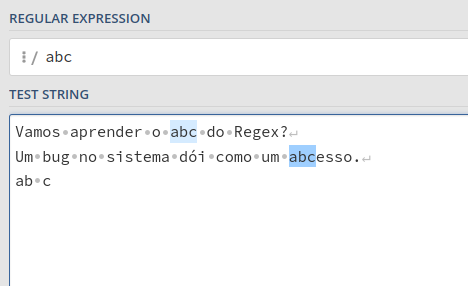
\includegraphics[width=0.8\textwidth]{./images/abc-match.png}
    \label{fig:abc-match} \\
    \textnormal{\fontsize{10pt}{12pt}Fonte: Autoria própria}
\end{figure}

\subsubsection{\underline{Expressão regular com metacaractere}}

Como mencionado anteriormente, quando se quer algo que é mais do
que uma simples correspondência direta, utilizam-se metacaracteres.
O caractere
\textbf{*}
é um metacaractere de expressão regular. Por exemplo:
\textbf{ab*c}
utiliza o
\textbf{*}
como metacaractere. A expressão
\textbf{ab*c}
deve ser lida como: Corresponda ao caractere
\textbf{a,}
seguido por zero ou mais caracteres
\textbf{b}s,
seguido por um caractere
\textbf{c.}
Usar
\textbf{*}
após o
\textbf{b}
significa: zero ou mais ocorrências do item anterior, no caso
\textbf{b.}
Como observa-se na
Figura \ref{fig:abc-meta-match}
as strings "cbbabbbbcdebc", "abbbbc"~ e "ac"~
encontrarão correspondências. As strings "ab", "a"~ e "abbbbbb", por
outro lado, não encontrarão correspondências, conforme a
Figura \ref{fig:abc-meta-not-match}.
\cite{mdn-regex}.

\begin{figure}[H]
    \centering
    \caption{Correspondêcias do Regex ab*c, com metacaractere}
    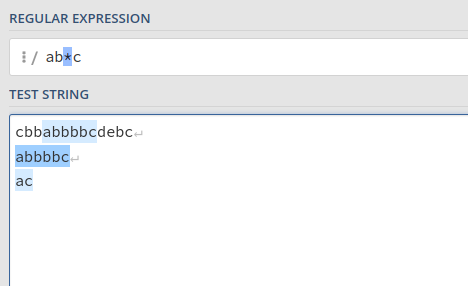
\includegraphics[width=0.8\textwidth]{./images/abc-meta-match.png}
    \label{fig:abc-meta-match} \\
    \textnormal{\fontsize{10pt}{12pt}Fonte: Autoria própria}
\end{figure}

\begin{figure}[H]
    \centering
    \caption{Não correspondêcias do Regex ab*c, com metacaractere}
    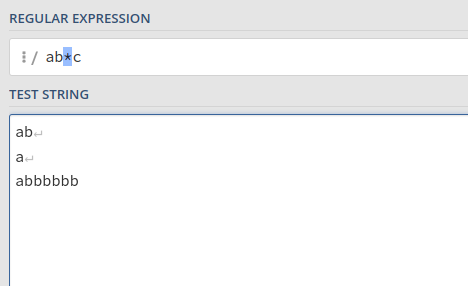
\includegraphics[width=0.8\textwidth]{./images/abc-meta-not-match.png}
    \label{fig:abc-meta-not-match} \\
    \textnormal{\fontsize{10pt}{12pt}Fonte: Autoria própria}
\end{figure}

Uma expressão regular é uma combinação de caracteres, alguns
deles, como o metacaractere quantificador *, visto
anteriormente, são caracteres especiais. Estes metacaracteres
são simbolos especiais que definem como a é interpretada.
\cite{dp6-regex}.

\subsubsection{\underline{Expressões regulares em JavaScript}}

Em JavaScript, as expressões regulares podem ser escritas diretamente dentro do código,
desde que postas entre barras //. Por exemplo: /abc/ é uma expressão regular válida em
\acrshort{js}.
O tipo de dados das expressões regulares é
o
\textit{object}\footnote{Do inglês: Objeto
}, assim como
\textit{Array}\footnote{Do inglês: Variedade ou matriz. No contexto de JavaScript é um dado estruturado,
    composto de uma sequencia de outros objetos ou dados puros.
}
ou
\textit{Set}\footnote{Do inglês: Conjunto. Assim como Array, é um dado estruturado que agrupa outros
    objetos, porém de forma não ordenada e não indexada.
}. As expressões regulares no
\acrshort{js}
são usadas com dois objetos principais, a saber
\acrshort{regex}
e
String.
A
\acrshort{api}
de strings do
\acrshort{js}
fornece uma gama de métodos nos quais se pode utilizar
juntamente com
\acrshort{regex}.
A Tabela \ref{tbl:string-methods-regex}
fornece uma descrição destes métodos:

\begin{table}[H]
    \centering
    \caption{Métodos de string que podem ser usados com regex}
    \label{tbl:string-methods-regex}
    \renewcommand{\arraystretch}{1.5}
    \begin{tabular}{p{2.4000cm} p{13.6000cm}}
        \hline
        \textbf{Método} & \textbf{Descrição} \\
        \hline
        match & O método match retorna o resultado da correspodência de um dado
            \cite{mdn-regex}
            à string ao qual está sendo aplicado. Aplicação em códido:
            "Meu abc".match(/abc/);
         \\
		matchAll & Faz o mesmo que match. Porém, ao contrário de match, que traz apenas
            a primeira correspondência, matchAll traz todas as correspondências
            encontradas.
         \\
		replace & O método replace de uma dada string, retorna uma nova string que substitui
            a correspondência de uma expressão regular por alguma string de substituição.
         \\
		replaceAll & Um caminho diferente para fazer o mesmo que replace, porém para todas
            as ocorrências.
         \\
		search & Faz uma busca pelo padrão na string e retorna o índice da primeira ocorrência. \\
		split & Divide a string em uma lista ordenada de substrings em que o critério de divisão é a expressão regular fornecida. \\
        \hline
        \\\multicolumn{2}{c}{\fontsize{10pt}{12pt}Fonte: \cite{mdn-regex}.}
    \end{tabular}
\end{table}

O objeto
\acrshort{regex}
também fornece dois métodos em que se usam as expressão regulares,
a saber: exec() e test().
\cite{mdn-regex}.

\subsection{Lamport Tex, LaTex}

O
\acrshort{latex}
é um sistema de preparação de documentos e processamento de texto,
desenvolvido na década de 1980 pelo norte-americano Leslie Lamport baseado
no sistema tipográfico TeX, desenvolvido por Donald Knuth.
\cite{latex-2}.

\vspace{15mm}
    \noindent
    \begin{minipage}{\textwidth}
        \noindent
        \begin{minipage}{4cm}
        \end{minipage}%
        \hfill
        \begin{minipage}{\dimexpr\textwidth-4cm}
            \hspace*{\parindent}
            \fontsize{10pt}{12pt}\selectfont % Ajusta o tamanho do texto para 10pt e altura da linha para 12pt
            O
\acrshort{latex}
é utilizado para criar documentos dos mais variados tipos de
publicação, como artigos, teses, dissertações, livros, cartas, relatórios ou qualquer
outro tipo de documento. Possui um alto grau de exatidão e precisão na diagramação do
conteúdo do documento e alta qualidade na formatação automática do documento. O
\acrshort{latex}
é uma ampliação do original sistema de tipografia TEX. Tornou-se um padrão
para produção de documentos científicos.
\cite{tutorial-latex}.
        \end{minipage}
    \end{minipage}
    \vspace{15mm}

O código escrito em
\acrshort{latex}
se utiliza de convenções de marcação (\textit{tagging}) para controlar o
modo como o texto é exibido, por exemplo: negrito, itálico, citação,
referências cruzadas e etc...
Sua utilidade está na produção de um texto entendível tanto por humanos,
quanto pela máquina que o compilará e formatará. Deste modo, o autor
pode ser distanciado da apresentação visual da informação, se preocupando
apenas com o conteúdo escrito.
\cite{latex-wiki}.

Observe como no exemplo da
Figura \ref{fig:latex-pdf}
o texto simples possui marcadores que demarcam sua exibição
no arquivo final. O marcador \textbackslash chapter demarca o capítulo, ao
passo que \textbackslash section uma subsessão, (ou sessão), do capítulo.
Uma das grandes utilidades é que tanto a enumeração já é feita
automaticamente, quanto sua presença no sumário já é automaticamente
preenchida.

\begin{figure}[H]
    \centering
    \caption{Exemplo de compilação de código LaTex}
    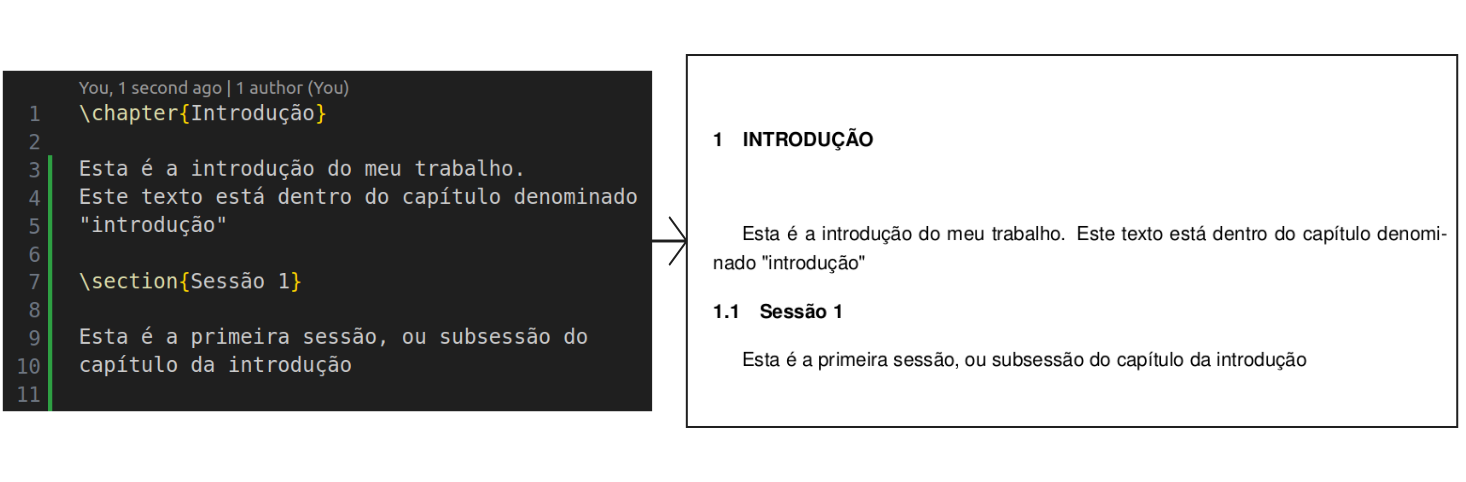
\includegraphics[width=1.0\textwidth]{./images/latex-pdf.png}
    \label{fig:latex-pdf} \\
    \textnormal{\fontsize{10pt}{12pt}Fonte: Autoria própria}
\end{figure}

\subsubsection{\underline{AbnTex2}}

\vspace{15mm}
    \noindent
    \begin{minipage}{\textwidth}
        \noindent
        \begin{minipage}{4cm}
        \end{minipage}%
        \hfill
        \begin{minipage}{\dimexpr\textwidth-4cm}
            \hspace*{\parindent}
            \fontsize{10pt}{12pt}\selectfont % Ajusta o tamanho do texto para 10pt e altura da linha para 12pt
            O abnTeX2, evolução do abnTeX (ABsurd Norms for TeX), é uma suíte para LaTeX que atende os requisitos das normas da
\acrshort{abnt}
(Associação Brasileira de Normas Técnicas) para elaboração de documentos técnicos e científicos brasileiros, como artigos científicos, relatórios técnicos, trabalhos acadêmicos como teses, dissertações, projetos de pesquisa e outros documentos do gênero.
 A suíte abnTeX2 é composta por uma classe, por pacotes de citação e de formatação de estilos bibliográficos, por exemplos, modelos de documentos e por uma ampla documentação.
 \cite{abntex2}
        \end{minipage}
    \end{minipage}
    \vspace{15mm}

\subsection{Cheerio}

Cheerio é uma biblioteca útil para processar linguagem de marcação.
Diferente do Browser, que renderiza uma página
\acrshort{html}
e implementa a estilização, Cheerio analisa a linguagem de marcação
tornando-a em dado estruturado. Deste modo, tem-se a possibilidade
de percorrer e manipular a estrutura de dados resultante do
código
\acrshort{html}.
Especificamente, o Cheerio não renderiza visualmente, aplica CSS,
carrega recursos externos ou executa JavaScript, o que é comum
em uma aplicação de página única
(\acrshort{spa},
na sigla em inglês).
Isso torna o Cheerio muito mais rápido do que outras soluções.

\subsubsection{\underline{Recursos}}

\begin{itemize}
        
	\item Sintaxe familiar: O Cheerio implementa um subconjunto do core do jQuery.
                O Cheerio elimina todas as inconsistências do
                \acrshort{dom}
                e as peculiaridades dos navegadores da biblioteca jQuery, revelando sua
                \acrshort{api}
                verdadeiramente esplêndida.
                
	\item Velocidade impressionante: O Cheerio trabalha com um modelo de 
                \acrshort{dom}
                muito simples e consistente. Como resultado, a análise, manipulação e renderização são incrivelmente eficientes.
                
	\item Incrivelmente flexível: O Cheerio utiliza o analisador parse5 e pode opcionalmente usar o tolerante htmlparser2 de @FB55. O Cheerio pode analisar praticamente qualquer documento
                \acrshort{html}
                ou
                \acrshort{xml}.
                
    
\end{itemize}

Fonte:
\cite{cheerio}

\chapter{Desenvolvimento}

A base da aplicação se dará por meio de um servidor onde serão realizadas
todas as operações. Este distribuirá o conteúdo estático e dinâmico
para a interação com o usuário, além também de fornecer rotas e funções
para o processamento do conteúdo gerado pelo usuário.
Por se tratar de uma aplicação em seu estágio inicial de concepção,
este projeto não se preocupará com autenticação e autorização de usuários.
Consistirá apenas de um servidor simples a ser rodado localmente a fim de
se desenvolver suas funcionalidades principais.

\section{O servidor NextJs}

O servidor da aplicação será construído em cima do NextJs, a
framewok React para a
\acrshort{web}.
Iniciar o projeto é uma tarefa simples. Basta apenas navegar
para algum diretório onde se deseja criar o projeto e
digitar o seguinte comando em
\acrshort{bash}\footnote{Bash (\textit{Bourne Again Shell}): Interface de linha de comando do linux
}:

\begin{createNextJsCommand}
npx create-next-app@latest
\end{createNextJsCommand}

Vale ressaltar que é necessário ter o NodeJs na versão 18.17 ou superior
para iniciar o projeto em NextJs. Após rodar este comando, o prompt fará uma
série de perguntas para a configuração do mesmo, observe o exemplo abaixo:

\begin{promptNextJs}
What is your project named? my-app
Would you like to use TypeScript? No / Yes
Would you like to use ESLint? No / Yes
Would you like to use Tailwind CSS? No / Yes
Would you like to use `src/` directory? No / Yes
Would you like to use App Router? (recommended) No / Yes
Would you like to customize the default import alias (@/*)? No / Yes
What import alias would you like configured? @/*
\end{promptNextJs}

Os itens a serem configurados são:

\begin{enumerate}
        
	\item Nome do projeto
	\item Será feito o uso de TypeScript?
	\item Será feito o uso de ESlint?
	\item Será feito o uso de Tailwind CSS?
	\item Será usado o diretório `src` como diretório padrão de código?
	\item Será utilizado o App Router (Roteador de App)?
	\item Deseja customizar o apelido padrão de importação (@/*)?
	\item Qual apelido de importação gostaria de configurar?
    
\end{enumerate}

A tabela
Tabela \ref{tbl:config-next-app}
mostra as opções escolhidas para este projeto:

\begin{table}[H]
    \centering
    \caption{Configurações do servidor NextJs}
    \label{tbl:config-next-app}
    \renewcommand{\arraystretch}{1.5}
    \begin{tabular}{p{13.0848cm} p{1.9552cm}}
        \hline
        \textbf{Pergunta} & \textbf{Resposta} \\
        \hline
        What is your project named? my-app & editor2 \\
		Would you like to use TypeScript? No / Yes & Yes \\
		Would you like to use ESLint? No / Yes & No \\
		Would you like to use Tailwind CSS? No / Yes & No \\
		Would you like to use `src/` directory? No / Yes & Yes \\
		Would you like to use App Router? (recommended) No / Yes & Yes \\
		Would you like to customize the default import alias (@/*)? No / Yes & Yes \\
		What import alias would you like configured? @/* & @/* \\
        \hline
        
    \end{tabular}
\end{table}

Os comandos a seguir instalam todas as dependências necessárias do projeto:

\begin{yarnAddDpts}
yarn add @editorjs/editorjs @editorjs/header @editorjs/list
yarn add -D @types/editorjs__header @types/node @types/react
yarn add @emotion/react @emotion/styled antd cheerio
yarn add -D @types/react-dom @types/uuid typescript 
yarn add node-latex react-icons uuid
\end{yarnAddDpts}

Após isso o utilitário de criação da aplicação NextJs
irá criar uma estrutura de pastas e arquivos de projeto
totalmente configurado e pronto para ser programado.
A
Figura \ref{fig:estrutura-basica-projeto}
mostra a estrutura de pastas base do projeto, com todos os seus respectivos
arquivos de configuração, roteamento e componentes básicos do react.

\begin{figure}[H]
    \centering
    \caption{Estrutura de pastas e arquivos básica do projeto}
    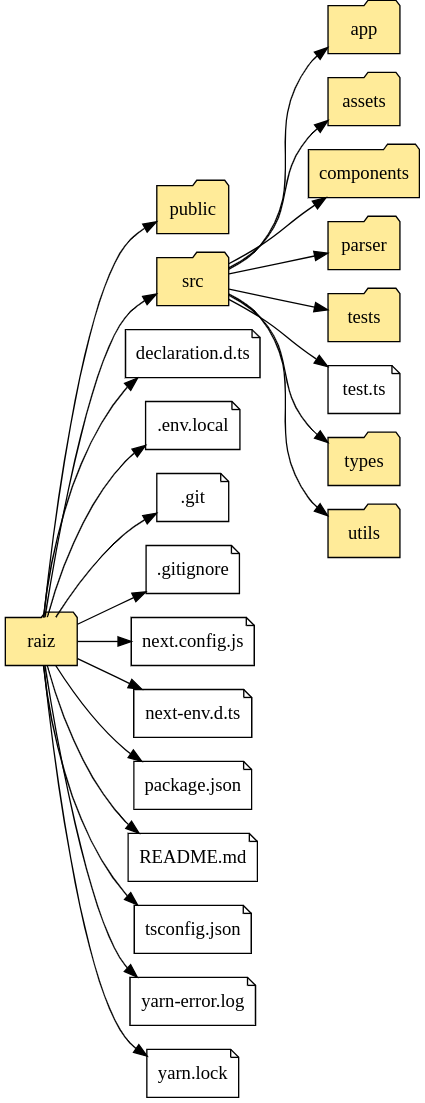
\includegraphics[width=0.4\textwidth]{./images/estrutura-basica-projeto.png}
    \label{fig:estrutura-basica-projeto} \\
    \textnormal{\fontsize{10pt}{12pt}Fonte: Autoria própria}
\end{figure}

\begin{table}[H]
    \centering
    \caption{Estrutura de pastas básica do projeto e suas atribuições}
    \label{tbl:pastas-projeto}
    \renewcommand{\arraystretch}{1.5}
    \begin{tabular}{p{3.2000cm} p{12.8000cm}}
        \hline
        \textbf{Arquivo/Pasta} & \textbf{Descrição} \\
        \hline
        public & Pasta pública para distribuição de arquivos estáticos. \\
		src & Esta pasta é praticamente
            o código fonte da aplicação onde todas as operações acontecem, tais
            quais: Edição com seus respectivos plugins; parser dos arquivos de
            saída e tudo mais.
         \\
		declaration.d.ts & Arquivo de declarações. Aqui é anotado algumas tipagens para serem usadas
            globalmente durante o processo de desenvolvimento.
         \\
		.env.local & Arquivo de variáveis de ambiente para serem usadas como teste durante                o tempo de desenvolvimento. \\
		.git & Pasta de controle do git. \\
		.gitignore & Arquivos a serem ignorados pela ferramenta de versionamento. \\
		next.config.js & Arquivo de configurações do NextJs. \\
		next-env.d.ts &  \\
		package.json & Arquivo que define que o projeto é um projeto NodeJs. Aqui está toda a informação sobre dependências
            do projeto, que são todos os pacotes usados de terceiros. Também possui definição
            de scripts úteis para serem utilizados no processo de desenvolvimento.
         \\
		README.md & Documentação de apresentação do projeto. \\
		tsconfig.json & Configurações do TypeScript. \\
		yarn-error.log & Erros do gerenciador de pacotes yarn \\
		yarn.lock & Arquivo de lock de dependências do gerenciador de pacotes yarn. \\
        \hline
        \\\multicolumn{2}{c}{\fontsize{10pt}{12pt}Fonte: Autoria própria}
    \end{tabular}
\end{table}

\subsection{Roteamento (App Router)}

No ato de configuração do servidor, conforme mostrado na
Tabela \ref{tbl:config-next-app},
na pergunta:
\textit{"Would you like to use App Router? (recommended) No / Yes"},
foi escolhida a opção sim, \textit{"yes"}.
Isto significa que no código fonte do projeto haverá uma pasta
chamada
\acrshort{app}
onde serão arquivados os roteamentos, as páginas,
layouts, páginas de erro, loading, entre outros.

A
Figura \ref{fig:app-router}
mostra a estrutura da pasta
\acrshort{app}.

\begin{figure}[H]
    \centering
    \caption{Estrutura da pasta de roteamento (App Router)}
    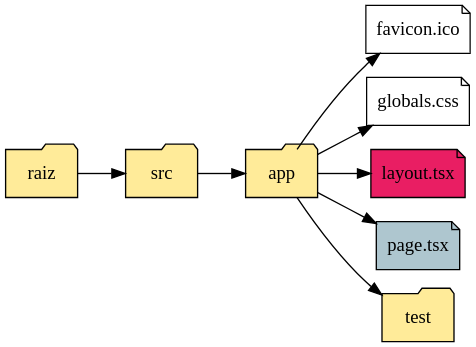
\includegraphics[width=0.8\textwidth]{./images/app-router.png}
    \label{fig:app-router} \\
    \textnormal{\fontsize{10pt}{12pt}Fonte: Autoria própria}
\end{figure}

Observe os arquivos destacados em azul e rosa, respectivamente
page.tsx e  layout.tsx. A extensão
\acrshort{tsx}
significa o mesmo que
\acrshort{jsx},
com a difereça de que é um arquivo em TypeScript ao
invés de JavaScript.

Os arquivos page e layout são a primeira página da aplicação.
Por estarem no nível do diretório
\acrshort{app} (dentro da pasta app)
esta página será mapeada para a rota / na navegação. Isto
significa que quando o servidor estiver rodando e o usuário
acessar o endereço do serviço, o código contido em
page.tsx renderizará o conteúdo da página para o
usuário.

O arquivo layout.tsx serve como um template para a página.
Pode-se pensá-lo como uma espécie de casca da aplicação.
A página herda o que está em layout, de modo que o que será
renderizado no Browser será o template, acrescido da page.

Por estar no diretório raiz de app, todas as rotas de páginas
da aplicação herdarão o que está em layout.tsx. Arquivos de 
layout também podem ser escritos em rotas que não sejam a raiz.

\subsubsection{\underline{Exemplo de criação de uma rota}}

Para criar uma rota para uma nova página no NextJs, basta que
uma pasta no diretótio app seja criada. Esta pasta deve conter
pelo menos um arquivo page.tsx ou route.ts. Observe a
Figura \ref{fig:page-route-example}.

\begin{figure}[H]
    \centering
    \caption{Estrutura da pasta de roteamento (App Router)}
    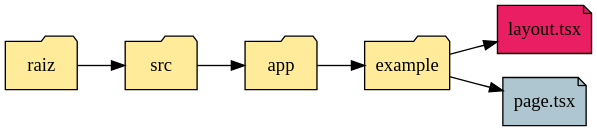
\includegraphics[width=0.8\textwidth]{./images/page-route-example.png}
    \label{fig:page-route-example} \\
    \textnormal{\fontsize{10pt}{12pt}Fonte: Autoria própria}
\end{figure}

Ao criar a pasta example com o arquivo page.tsx. O servidor
mapeará para a rota /example no Browser, renderizando o componente
exportado em page. Observe a seguir o código em layout.tsx:

\begin{layoutExample}
import { PropsWithChildren } from "react";

export default function Layout(
    { children }: PropsWithChildren
){
    return <section>
        <h1>Eu sou o Layout</h1>
        { children }
    </section>
}
\end{layoutExample}

Observe que o arquivo exporta uma função
denominada Layout, que retorna um código
\acrshort{tsx}
a ser renderizado na página.
Na linha 4 a função recebe um objeto
como parâmetro que é anotado por PropsWithChildren.
Dentro deste objeto há a propriedade
\textit{children}\footnote{Do inglês: Filhos.
},
que
contém outros componentes React a serem renderizados.
No caso, o NextJs injetará dentro de children o código que
é exportado por page.tsx.
A linha 8 é a posição onde este componente será renderizado.

Observe abaixo o código de page.tsx:

\begin{pageExample}
export default function Page(){
    return <div>
        Olá mundo!
        Eu sou uma page.
    </div>
}
\end{pageExample}

No código page apenas é exportada uma função (componente)
Page que retorna uma frase simples: "Olá mundo! Eu sou uma page".

\subsubsection{\underline{Executando o exemplo}}

Para executar o exemplo e ver como ele se comporta no navegador
do usuário, basta a partir do diretório do projeto rodar o
seguinte comando:

\begin{ee65bca1a1874d3fb302b1f4b7cf8a96}
yarn dev
\end{ee65bca1a1874d3fb302b1f4b7cf8a96}

Após rodar o comando o servidor iniciará localmente.
A saída do terminal mostrará a porta do serviço a ser acessada
afim de renderizar a página:

\begin{Code4d5f06a4f0c74be78e79a16da9033e18}
yarn run v1.22.19
$ next dev
    Next.js 14.1.1
    - Local:        http://localhost:3000
    - Environments: .env.local

    Ready in 2.7s
\end{Code4d5f06a4f0c74be78e79a16da9033e18}

Ao acessar o endereço http://localhost:3000
na rota /example, a página é renderizada
conforme a
Figura \ref{fig:example-route}:

\begin{figure}[H]
    \centering
    \caption{Exemplo de roteamento}
    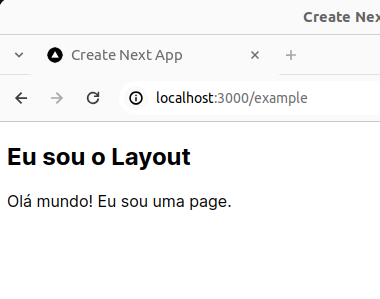
\includegraphics[width=0.6\textwidth]{./images/example-route.png}
    \label{fig:example-route} \\
    \textnormal{\fontsize{10pt}{12pt}Fonte: Autoria própria}
\end{figure}

\subsection{Página principal}

Neste primeiro momento, o editor em que o usuário interagirá
será renderizado na página principal. Conforme dito anteriormente
e ilustrado na
Figura \ref{fig:app-router},
a página principal está contida ao nível da pasta app, juntamente com
seu layout.

\subsubsection{\underline{Layout}}

O arquivo de layout é o template base no qual todas as outras páginas herdarão.
Observe na
Figura \ref{fig:layout-render-tree}
a sub árvore de renderização do layout:

\begin{figure}[H]
    \centering
    \caption{Sub árvore de renderização do layout principal}
    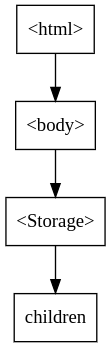
\includegraphics[width=0.1\textwidth]{./images/layout-render-tree.png}
    \label{fig:layout-render-tree} \\
    \textnormal{\fontsize{10pt}{12pt}Fonte: Autoria própria}
\end{figure}

Tem-se uma estrutura básica com a tag html, (a tag raiz do documento),
logo após o body, que diz respeito à área de renderização do documento.
Storage é um componente personalizado em React que será discutido mais adiante,
ele serve basicamente para armazenar conteúdos no navegador do usuário.
Logo em seguida há o último componente, (ou nó folha), que consiste no
children. Neste contexto, children pode ser qualquer coisa a depender
da rota de página ao qual se está acessando.

Observe abaixo o código de layout:

\begin{Code12a2e04935ad4280add32b616b8e09b9}
import type { Metadata } from 'next'
import { Inter } from 'next/font/google'

import Storage from '@/components/Storage';

const inter = Inter({ subsets: ['latin'] })

export const metadata: Metadata = {
    title: 'Create Next App',
    description: 'Generated by create next app',
}

export default function RootLayout({
    children,
}: {
    children: React.ReactNode
}) {
    return (
        <html lang="pt-BR">
            <body className={inter.className}>
                <Storage>
                    {children}
                </Storage>
            </body>
        </html>
    )
}
\end{Code12a2e04935ad4280add32b616b8e09b9}

Na linha 13 há a exportação do componente em si. O código
\acrshort{tsx}
é retornado a partir da linha 18.
Note que aqui não há o uso da tag head, padrão comum do
\acrshort{html}. Isso se dá
pois o gerenciamento das configurações desta tag fica
a cargo do NextJs. Nas linhas 8 à 11
há a exportação de uma constante denominada metadata. Nela
há a chave title que o Next utilizará para renderizar o
título da página, (que em um html normal seria configurado
dentro de head).

\subsubsection{\underline{Page}}

O arquivo page.tsx exporta o componente React denominado Home,
que é a tela inicial propriamente dita.
Embora os componentes em React sejam definidos como funções,
os mesmos serão representados em forma de diagrama de
classes para fins didáticos. Toda representação de
componente terá um método render() que retorna um código
\acrshort{jsx}. Este método
não existe no componente em si, mas sim na implementação
do React. Pode-se pensar o render() como a função que
renderiza o que é retornado pela "função componente"~
Home.
A
Figura \ref{fig:class-home-component}
ilustra o componente em forma de diagrama de classe com seus estados e utilitários.

\begin{figure}[H]
    \centering
    \caption{Componente da página Home}
    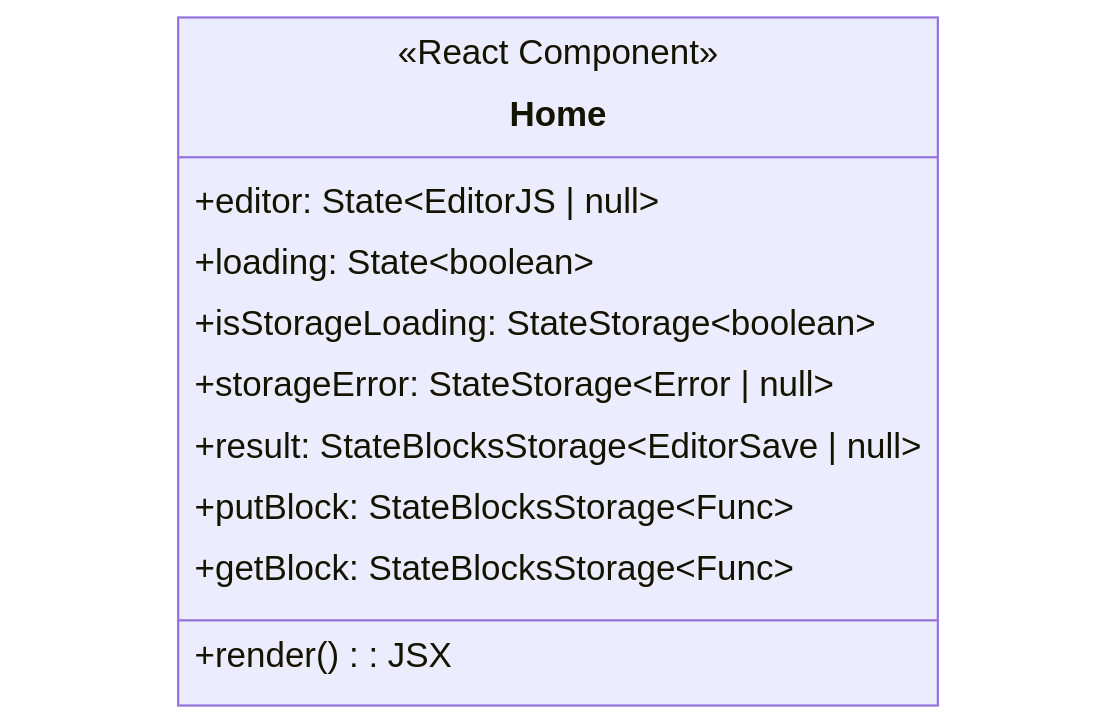
\includegraphics[width=0.7\textwidth]{./images/class-home-component.png}
    \label{fig:class-home-component} \\
    \textnormal{\fontsize{10pt}{12pt}Fonte: Autoria própria}
\end{figure}

O campo editor é o mais importante de todos, pois é nele
que estará armazanada a referência à classe EditorJs em forma de estado.
É importante salientar que todo estado vem acompanhado com uma função
de atualização. Sempre que este estado é atualizado, a função de renderização
é chamada novamente, remotando o componente e consequentemente todas as referências
aos seus estados.

Note que o campo editor pode ser uma instância de EditorJs ou um valor nulo.
Isso se dá pois inicialmente este estado começa nulo até que a classe seja
carregada.
Observe na
Figura \ref{fig:page-render-tree}
como o componente Home será renderizado:

\begin{figure}[H]
    \centering
    \caption{Sub árvore de renderização da página principal}
    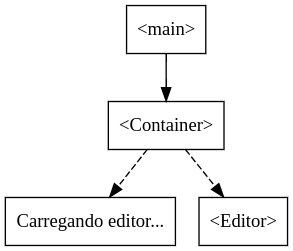
\includegraphics[width=0.5\textwidth]{./images/page-render-tree.png}
    \label{fig:page-render-tree} \\
    \textnormal{\fontsize{10pt}{12pt}Fonte: Autoria própria}
\end{figure}

Percebe-se que o componente Container possuí dois filhos: Um texto
("Carregando editor...") e o componente Editor.
Observe a partir da linha 87 no código abaixo como a renderização
do texto "Carregando editor..."~ está condicionada ao estado loading.

\begin{Code40b89bba73044d838c6a511b43954ee7}
[...]
return (
    <main>
        <Container>
            {
                loading
                    ? 'Carregando editor...'
                    : null
            }
            <Editor
[...]
\end{Code40b89bba73044d838c6a511b43954ee7}

O estado loading inicialmente começa com o valor true, o que
faz com que o texto seja renderizado. O componente
Editor também estará em tela, mas como faz uso da classe EditorJs,
só aparecerá quando a mesma estiver pronta.

Note na linha 121 do código abaixo que a propriedade
\textit{onReady}\footnote{Do inglês: Quando pronto.
},
que pertence ao componente Editor, recebe uma função
com o parâmetro \{ editor \}.

\begin{Code14581fc6c8e549c29960fa25e3c62563}
[...]
onReady={ ({ editor }) => {
    setLoading(false);
    setEditor(editor);
} }
[...]
\end{Code14581fc6c8e549c29960fa25e3c62563}

A propriedade onReady é um evento que chama
a função passada quando a classe EditorJs está pronta e
totalmente carregada. Note que a função passada chama dois
atualizadores de estado: setLoading e setEditor. Estes atualizadores
setam\footnote{Neologismo derivado do verbo inglês 'To Set' que significa 'Definir',
    \cite{setar}.
}
os estados loading como false, e editor com o valor \{ editor \} presente
no parâmetro da função. O resultado disso é que a partir deste momento
o texto ("Carregando editor...") não aparecerá mais em tela; o editor
estará pronto para ser usado; e o estado editor possui a referência
à classe com toda a
\acrshort{api}
do EditorJs.

A
            Tabela \ref{tbl:props-componente-home}
            lista cada um dos estados do componente Home, bem como cada uma de suas
            atribuições:

\begin{table}[H]
    \centering
    \caption{Propriedades do componente de tela Home}
    \label{tbl:props-componente-home}
    \renewcommand{\arraystretch}{1.5}
    \begin{tabular}{p{3.5200cm} p{2.8800cm} p{9.6000cm}}
        \hline
        \textbf{Propriedade} & \textbf{Atualizador} & \textbf{Descrição} \\
        \hline
        editor & setEditor & Armazena a referência à classe do EditorJs \\
		loading & setLoading & Estado de quando a tela está carregando \\
		isStorageLoading & Automático & Quando a \acrshort{api}                    da Storage está carregando \\
		storageError & Automático & Caso haja algum erro com a Storage \\
		result & Automático & Blocos guardados na Storage, (caso Hajam) \\
		putBlock & Automático & Função para guardar blocos na Storage \\
		getBlock & Automático & Função para pegar blocos da Storage \\
        \hline
        \\\multicolumn{3}{c}{\fontsize{10pt}{12pt}Fonte: Autoria própria}
    \end{tabular}
\end{table}

\subsubsection{\underline{Disparo de efeitos}}

Os estados podem alterar o comportamento da tela, bem como seu fluxo de renderização
de modo a enriquecer a experiência de usuário. A mudança de um estado também pode
disparar um efeito. Efeito este que adiciona alguma ação ou modificação de outros estados.
Observe o código abaixo:

\begin{Code6d60f882aea34cf68d9c6f6ca7c992ff}
[...]
useEffect(() => {
    if(storageError){
        console.error('Storage error', storageError);
        message.error('Erro ao carregar storage');
    }
}, [ storageError ]);
[...]
\end{Code6d60f882aea34cf68d9c6f6ca7c992ff}

O código acima adiciona uma função que monitora o estado denominado
storageError. Na primeira renderização da página, ou sempre que este
estado muda, a função é disparada. Tudo que a função faz é checar se há
algum erro presente em storageError. Caso afirmativo, o erro é transcrito
na saída de erro do console através da linha 78, e uma mensagem
é exibida ao usuário na linha 79.
A
Figura \ref{fig:effect-storageError}
ilustra este comportamento de forma visual:

\begin{figure}[H]
    \centering
    \caption{Disparo de efeito de storageError}
    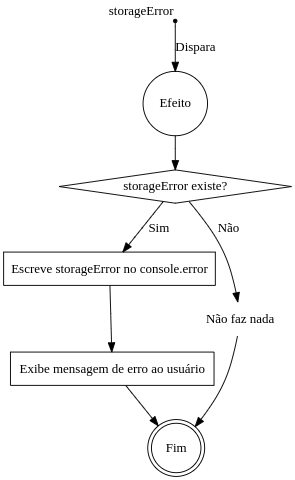
\includegraphics[width=0.5\textwidth]{./images/effect-storageError.png}
    \label{fig:effect-storageError} \\
    \textnormal{\fontsize{10pt}{12pt}Fonte: Autoria própria}
\end{figure}

Diversos efeitos podem ser adicionados ao longo do componente, e cada
efeito pode monitorar um ou mais estados. Observe na
Figura \ref{fig:effect-editor-result}
como os estados
result e editor se utilizam de um efeito para checar se existem blocos
salvos para então carregá-los através da
\acrshort{api}
contida em editor:

\begin{figure}[H]
    \centering
    \caption{Disparo de efeito de result e editor}
    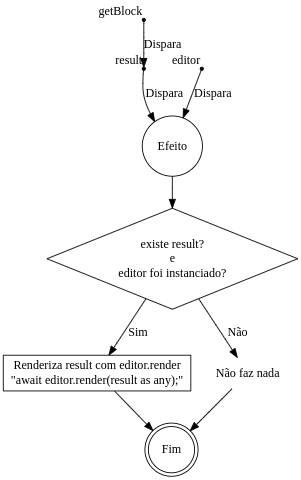
\includegraphics[width=0.7\textwidth]{./images/effect-editor-result.png}
    \label{fig:effect-editor-result} \\
    \textnormal{\fontsize{10pt}{12pt}Fonte: Autoria própria}
\end{figure}

Note como getBlock, que é uma função provida pelos estados do BlockStorage,
pode disparar uma mudança no estado result. Este é exatamente o fluxo desejado.
A
Figura \ref{fig:effect-isStorageLoading}
mostra como a aplicação fica aguardando a Storage carregar, e assim
que ela carrega, getBlock é chamada, disparando o result, que porventura
seguirá o fluxo na
Figura \ref{fig:effect-editor-result}.

\begin{figure}[H]
    \centering
    \caption{Disparo de efeito isStorageLoading}
    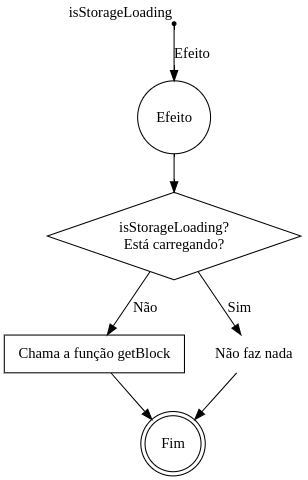
\includegraphics[width=0.5\textwidth]{./images/effect-isStorageLoading.png}
    \label{fig:effect-isStorageLoading} \\
    \textnormal{\fontsize{10pt}{12pt}Fonte: Autoria própria}
\end{figure}

Por fim, a função putBlock é utilizada por um evento disparado
pelo componente Editor. Observe como a propriedade
\textit{onChange}\footnote{Do inglês: Quando mudar
}
recebe uma função que recupera o estado atual do editor, e em
seguida repassa-o para putBlock.

Os detalhes de implementação da Storage se encontram no repositório através
do diretório: /src/components/Storage

\begin{Codee84c5b55b5f94df497da8049aeb02dac}
[...]
onChange={async (api, event) => {
    const blocks = await api.saver.save();
    putBlock(blocks as EditorSave);
}}
[...]
\end{Codee84c5b55b5f94df497da8049aeb02dac}

\section{Editor}

O Editor é o principal componente da aplicação em termos de interatividade
com o usuário e
\acrshort{ux}.
Através dele o usuário poderá inserir os blocos a comporem o seu trabalho acadêmico.
Veja na
Figura \ref{fig:estrutura-editor-componente}
a localização da estrutura de pastas no projeto.

\begin{figure}[H]
    \centering
    \caption{Estrutura de pastas do componente Editor}
    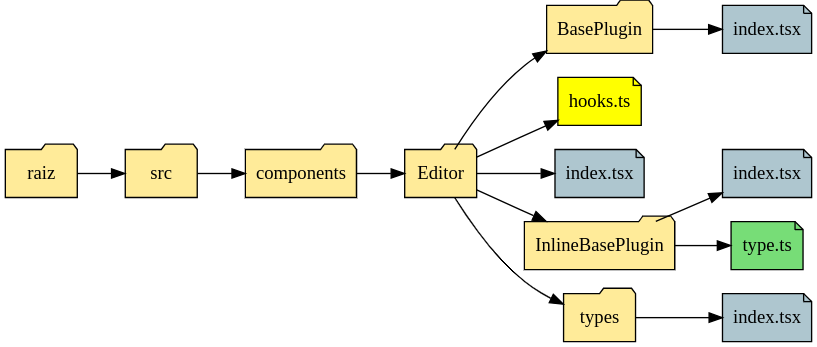
\includegraphics[width=0.9\textwidth]{./images/estrutura-editor-componente.png}
    \label{fig:estrutura-editor-componente} \\
    \textnormal{\fontsize{10pt}{12pt}Fonte: Autoria própria}
\end{figure}

\subsection{Provider}

O componente do Editor propriamente dito, aqui denominado
Provider, é exportado pelo arquivo Editor/index.tsx. É Chamado de
Provider pois em seu contexto são colocadas funções que poderão ser
utilizadas no decorrer de toda a aplicação, com a condição de que os componentes
utilizadores sejam filhos de Editor.
A
Figura \ref{fig:class-editor-component}
contém a descrição do componente:

\begin{figure}[H]
    \centering
    \caption{Componente React - Editor}
    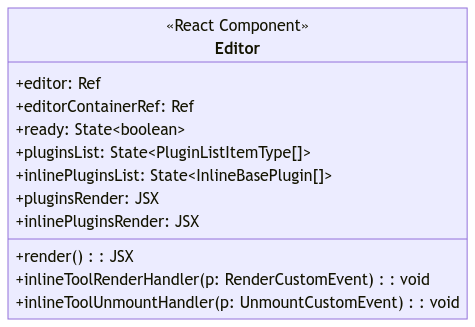
\includegraphics[width=0.6\textwidth]{./images/class-editor-component.png}
    \label{fig:class-editor-component} \\
    \textnormal{\fontsize{10pt}{12pt}Fonte: Autoria própria}
\end{figure}

Os dois principais atributos deste componente são: editor e editorContainerRef,
ambos anotados como Ref.
Desta vez, estes atributos não são estados, mas sim referências. A referência,
ao contrário do estado não possui função de atualização. São objetos especiais
que podem guardar referências para objetos no
\acrshort{dom}
ou outros objetos JavaScript. Isso acontece pois editor guardará a instância
do EditorJs, ao passo que editorContainerRef referenciará uma div no
\acrshort{dom}.
Esta div será utilizada por editor para inputar a ferramenta de edição de
texto.

Observe na
Figura \ref{fig:sub-tree-render-editor}
que o Context.Provider renderiza dois elmentos div irmãos. O azul, que conterá
os plugins nomais e in-line. E o vermelho que é a div na qual se define
o atributo ref com editorContainerRef.

\begin{figure}[H]
    \centering
    \caption{Sub árvore de renderização do componente Editor}
    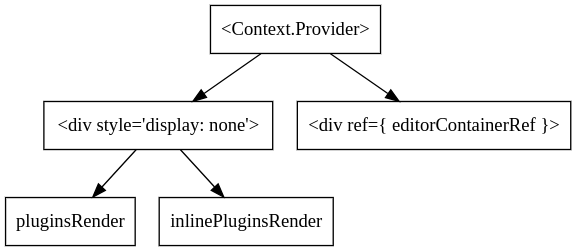
\includegraphics[width=0.7\textwidth]{./images/sub-tree-render-editor.png}
    \label{fig:sub-tree-render-editor} \\
    \textnormal{\fontsize{10pt}{12pt}Fonte: Autoria própria}
\end{figure}

Observe que a div azul não é exibida em tela através da propriedade
style='display: none'. Isso acontece porque os plugins listados
nela serão transportados para dentro da div vermelha por meio de
um conceito chamado \textit{React Portals}. Virtualmente, para o React,
os plugins estarão na div azul. Porém praticamente, eles estarão na verdade
dentro da div vermelha num lugar a ser definido pelo EditorJs, que define
isso automaticamente. Este recurso é usado para se injetar os componentes
do React dentro do editor sem quebrar sua árvore lógica. Mais a frente
será demonstrado que a classe EditorJs é quem é responsável por chamar
e decidir a localização de cada componente através da
instanciação de classes.

A
Figura \ref{fig:effect-ready-editor-component}
ilustra o processo simplificado de quando o estado ready é disparado.
Ready é disparado quando acontece a primeira renderização da página, por meio
de um efeito que não monitora nenhum estado em particular. A tarefa deste efeito
é apenas setar o estado ready para true. Isto funciona pois o efeito que
não monitora nenhum estado é executado apenas uma vez, quando o componente é
renderizado.

\begin{figure}[H]
    \centering
    \caption{Simplificação do Efeito ready no componente Editor}
    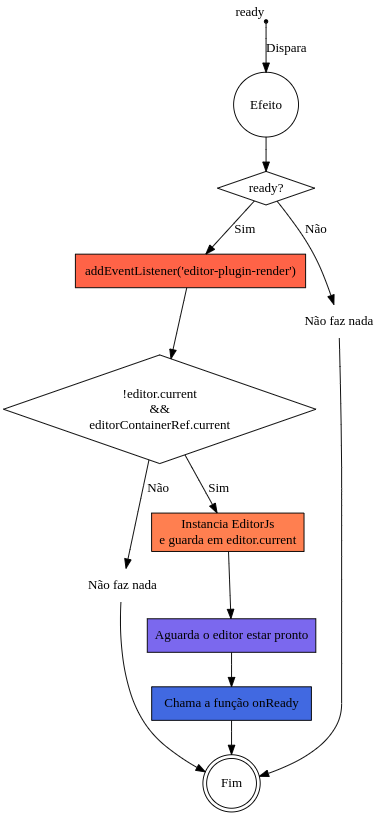
\includegraphics[width=0.7\textwidth]{./images/effect-ready-editor-component.png}
    \label{fig:effect-ready-editor-component} \\
    \textnormal{\fontsize{10pt}{12pt}Fonte: Autoria própria}
\end{figure}

\subsubsection{\underline{Event Listener}}

O quadro vermelho na
Figura \ref{fig:effect-ready-editor-component}
corresponde a adição de um escutador de
evento personalizado denominado \textit{editor-plugin-render}.
Isto é importante pois este evento recebe a criação dos plugins que
são disparados de dentro da classe EditorJs. Observe o código abaixo:

\begin{Code9ca9d3091ea34f6e8398f3e033b9d5f5}
[...]
document.addEventListener('editor-plugin-render', e => {
    // console.log('editor-plugin-render');
    // console.log({ e });
    setPluginsList(prev => [
        ...prev,
        {
            excluded: false,
            // @ts-ignore
            plugin: e.detail.context
        }
    ]);
});
[...]
\end{Code9ca9d3091ea34f6e8398f3e033b9d5f5}

Na linha 137 o escutador é adicionado ao objeto
\acrshort{dom}. Este evento monitora
qualquer renderização de plugin que é despachada, seja ela da onde
for. Quando acontece um despache a função é chamada, de modo que na linha
140 tem-se a adição do plugin na lista de plugins.
Note que o objeto adicionado possui uma propriedade excluded
que controla quando o plugin sai de cena.

Quando o estado
pluginsList
é atualizado por setPluginsList, a lista de plugins
é memorizada em pluginsRender, que é então
renderizado na linha 213 do código abaixo:

\begin{Code12863a1c5215452288034462c425678a}
[...]
    return <Context.Provider value={{
        editor: editor.current
    }}>
        <div style={{ display: 'none' }}>
            { pluginsRender }
            { inlinePluginsRender }
        </div>
        <div ref={ editorContainerRef } ></div>
    </Context.Provider>
}
\end{Code12863a1c5215452288034462c425678a}

\subsubsection{\underline{Instância do EditorJs}}

Os quadros laranja, violeta e azul da
Figura \ref{fig:effect-ready-editor-component}
correspondem a instanciação do EditorJs e suas configurações.
Quando a referência editor ainda não foi atribuida mas o editorContainerRef
já está renderizado em tela conforme a linha 173, a linha 175 se encarrega
de instanciar a classe EditorJS.

Observe a importancia da linha 177 em que a referência editorContainerRef
é repassada para a propriedade holder. O EditorJS utiliza essa propriedade para
colocar a ferramenta de edição na
\acrshort{dom}
através da referência ao elemento repassado.

A propriedade tools recebe o register na linha 178, que nada mais é do que a lista
de plugins repassada quando o componente vai ser utilizado.
na linha 190 há uma espécie de trava que aguarda até que o editor esteja pronto
antes de chamar a função onReady na linha 192. Note que onReady só é chamada caso
a mesma tenha sido repassada. Ao chamar, a instância do editor é repassada na linha
193.

\begin{Codef42fa1a75c7f4d44af80606a175bb37b}
[...]
if(!editor.current && editorContainerRef.current){
    // console.log("Comming to assing editorjs...");
    editor.current = new EditorJS({
        ...config,
        holder: editorContainerRef.current,
        tools: Object.keys(register).reduce((prev, key) => {
            const { component, ...restOfProps } = register[key];
            return {
                ...prev,
                [key]: restOfProps
            };
        }, {}),
        onChange: (api, event) => {
            onChange && onChange(api, event);
        },
    });

    await editor.current.isReady;

    onReady && onReady({
        editor: editor.current
    })
}
[...]
\end{Codef42fa1a75c7f4d44af80606a175bb37b}

\subsection{BasePlugin}

A classe BasePlugin será a classe na qual todos os plugins irão derivar.
Ela implementa os métodos chamados pelo EditorJS quando um plugin customizado
é chamado pela
\acrshort{api}
do EditorJS.

\begin{figure}[H]
    \centering
    \caption{Classe - BasePlugin}
    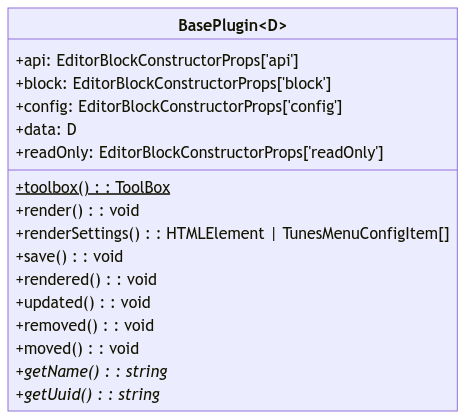
\includegraphics[width=0.6\textwidth]{./images/class-base-plugin.png}
    \label{fig:class-base-plugin} \\
    \textnormal{\fontsize{10pt}{12pt}Fonte: Autoria própria}
\end{figure}

A tabela
Tabela \ref{tbl:base-plugin-methods}
mostra a descrição dos métodos da classe e suas atribuições.

\begin{table}[H]
    \centering
    \caption{Métodos da classe BasePlugin}
    \label{tbl:base-plugin-methods}
    \renewcommand{\arraystretch}{1.5}
    \begin{tabular}{p{5.6000cm} p{10.4000cm}}
        \hline
        \textbf{Método} & \textbf{Descrição} \\
        \hline
        toolbox() & Método estático que retorna o ícone do plugin a ser renderizado no menu \\
		render() & Método que renderiza o plugin na ferramenta de edição
             \\
		renderSettings() & Método que renderiza o menu personalizado do plugin
             \\
		save() & Método que retorna o estado do componente quando saver da
                \acrshort{api}
                é chamado
             \\
		redered() & Método disparado quando o plugin é renderizado
             \\
		updated() & Método disparado quando o plugin é atualizado
             \\
		removed() & Método disparado quando o plugin é removido
             \\
		moved() & Método disparado quando o plugin é movido
             \\
		getName() & Método abstrado que retorna o nome do Plugin.
                Toda implementação de plugin deve implementar essa
                classe obrigatoriamente
             \\
		getUuid() & Método abstrado que retorna um identificador único ao instanciar o plugin.
                Toda implementação de plugin deve implementar essa
                classe obrigatoriamente
             \\
        \hline
        
    \end{tabular}
\end{table}

O método mais importante da classe base é o render(). É ele quem coloca o plugin
em tela quando o usuário escolhe um plugin a partir do menu de plugins.
Observe no código abaixo o funcionamento da classe:

\begin{Code35cc7dfc86bb420587d75d1c81a7cb0e}
[...]
public render(){
    const wrapper = document.createElement('div');
    wrapper.id = this.pluginId;

    const ev = new CustomEvent<{ context: BasePlugin }>(
        'editor-plugin-render', {
            detail: {
                context: this
            }
        }
    );
    setTimeout(() => document.dispatchEvent(ev), 20);

    return wrapper;
}
[...]
\end{Code35cc7dfc86bb420587d75d1c81a7cb0e}

Observe que o método render cria um wrapper a partir de um elemento
div na linha 52. Na linha 53 é atribuído um id a partir da chamada do método
getUuid(). Na linha 55 a 61 é criado um evento customizado que é despachado
20 milissegundos após o retorno do wrapper.
O wrapper é o que o EditorJS renderiza na ferramenta. O despache do evento
juntamente com a referência à instância da classe é então capturada pelo
escutador discutido na
Figura \ref{fig:effect-ready-editor-component}
da sessão Provider. Assim, o plugin do react vai para a lista de plugins ao mesmo
tempo que é renderizado de forma integrada ao EditorJS.
(Falar do código do portal)

\subsection{Plugins}

Plugins são o principal objetivo em se usar o EditorJS, pois cada plugin é o que
se traduz nos blocos da escrita em blocos conceituada no capítulo 1.
A
Figura \ref{fig:estrutura-plugins}
ilustra a estrutura de pastas dos plugins que foram desenvolvidos:

\begin{figure}[H]
    \centering
    \caption{Estrutura de pastas dos plugins}
    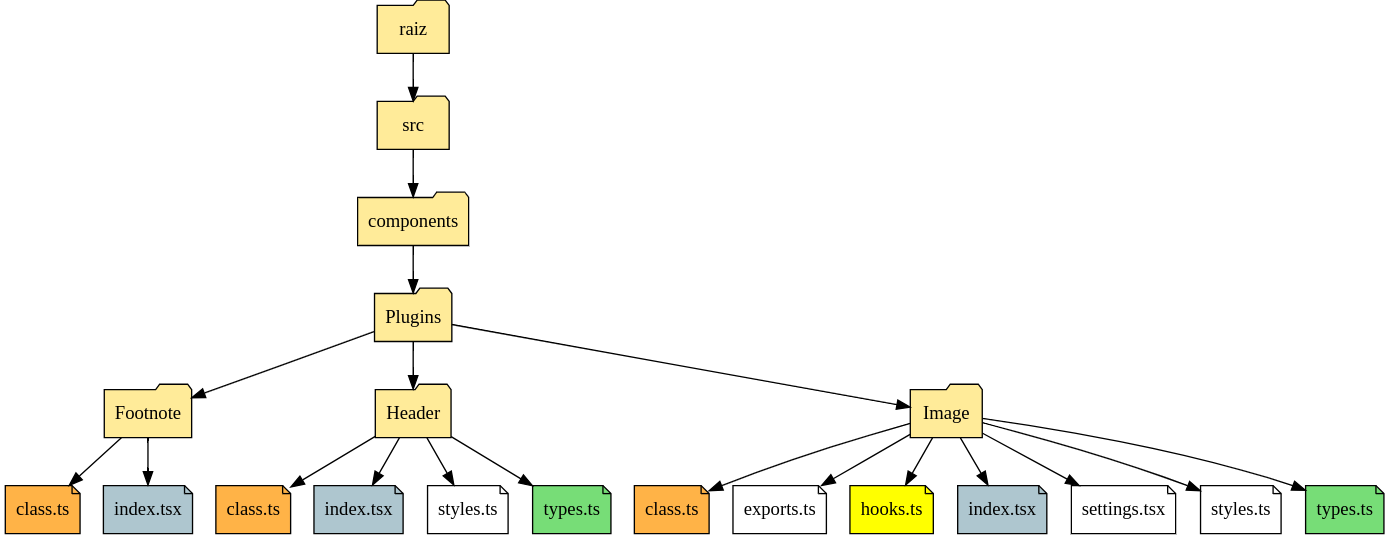
\includegraphics[width=1.0\textwidth]{./images/estrutura-plugins.png}
    \label{fig:estrutura-plugins} \\
    \textnormal{\fontsize{10pt}{12pt}Fonte: Autoria própria}
\end{figure}

Observe que as condições mínimas para a existência de um plugin é possuir
os arquivos index.tsx e class.ts. O arquivo class.ts é a classe propriamente
dita que é derivada de BasePlugin, que consequentemente há de se implementar
os dois métodos abstratos obrigatórios.

O arquivo index.tsx é o componente React interativo. É neste arquivo em que
se programa a aparência e comportamentos do mesmo.

\subsubsection{\underline{Header}}

O plugin de Header, (até o momento de escrita deste trabalho), pode ser considerado um dos mais simples
que foi desenvolvido. Observe abaixo a implementação do arquivo class.tsx:

\begin{Code11e75fa498f94562ab38221213644802}
[...]
export default class HeaderClass extends BasePlugin<DataType> {
    text: string = ""
    public setLevel:
        Dispatch<SetStateAction<HeaderLevelsType>> | null = null

    static get conversionConfig() {
        return {
            export: 'text',
            import: 'text',
        };
    }
[...]
\end{Code11e75fa498f94562ab38221213644802}

Na linha 17, é realizada a exportação da classe HeaderClass,
que estende a classe BasePlugin. Observe que nas linhas 18 e 19,
são definidas uma propriedade text (que armazenará o texto do Header)
e a função setLevel (que é uma função de atualização de estado do React).

No caso do plugin Header, é importante ter uma referência à função
de atualização do nível (level) do Header, pois é nesta classe que
o menu, onde o usuário selecionará o nível do título, é definido,
conforme o código abaixo:

\begin{Code48a69fa7e0f2483b9c8309a2cc169afb}
[...]
public renderSettings(): TunesMenuConfigItem[] {
    return ([1,2,3,4,5] as HeaderLevelsType[]).map(lv => ({
        title: `Nível ${lv}`,
        // @ts-ignore
        onActivate: () => {
            console.log({ setLevel: this.setLevel });
            this.setLevel && this.setLevel(lv);
        },
        closeOnActivate: true,
        isActive: lv === this?.pluginData?.level,
[...]
\end{Code48a69fa7e0f2483b9c8309a2cc169afb}

Observe como a função de atualização de estado é chamada a partir de onActivate
na linha 40. Isso garante a comunicação do menu com o componente React, permitindo
ao usuário selecionar o nível de título a partir do menu.

No código abaixo tem-se a implementação das duas funções abstratas obrigatórias
getName() e getUuid(). Observe que em getName retorna-se o nome header do plugin,
ao passo que em getUuid retorna-se um uuid versão 4 para criar um identificador
único para o plugin.

\begin{Code7a9dec7aa71746cc81a8bc51cb6697a6}
[...]
    getName(): string {
        return 'header';
    }

    getUuid(): string {
        return uuidv4();
    }
}
\end{Code7a9dec7aa71746cc81a8bc51cb6697a6}

\subsubsubsection{Plugin React}

\begin{figure}[H]
    \centering
    \caption{Plugin: Componente React}
    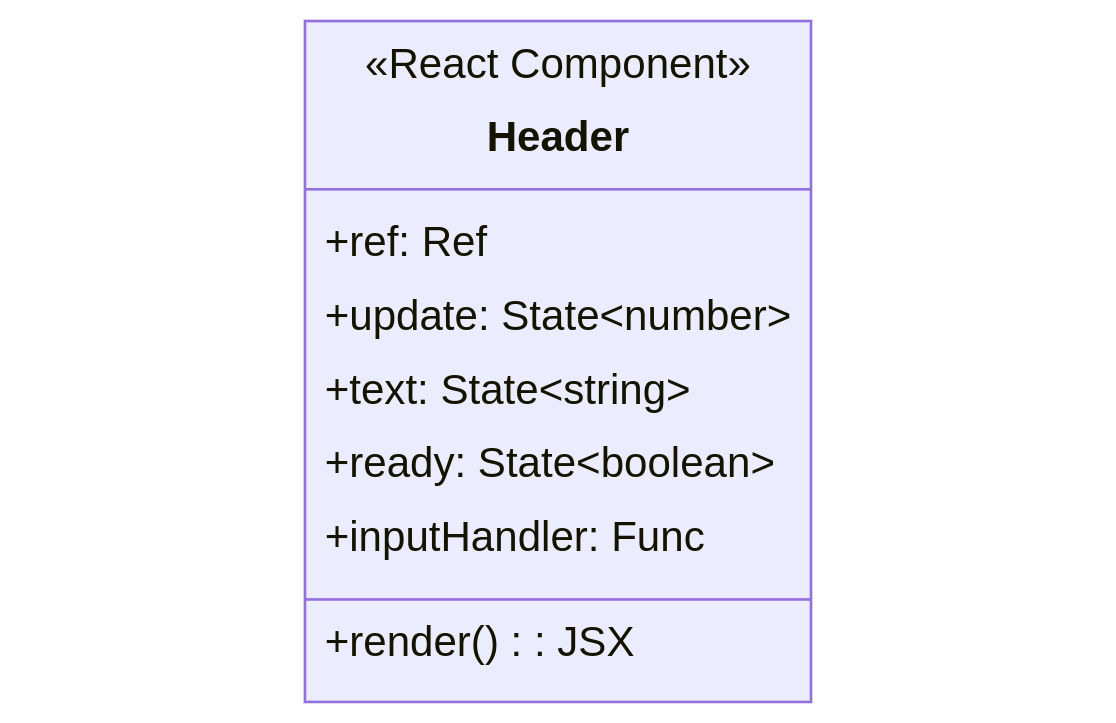
\includegraphics[width=0.7\textwidth]{./images/header-plugin-component.png}
    \label{fig:header-plugin-component} \\
    \textnormal{\fontsize{10pt}{12pt}Fonte: Autoria própria}
\end{figure}

\subsubsubsection{Aparência}

A
Figura \ref{fig:show-header}
mostra como o plugin de Header se parece na interface do editor.
Também é possível observar seus subtítulos juntamente blocos de
parágrafo.

\begin{figure}[H]
    \centering
    \caption{Plugin de Header na interface gráfica}
    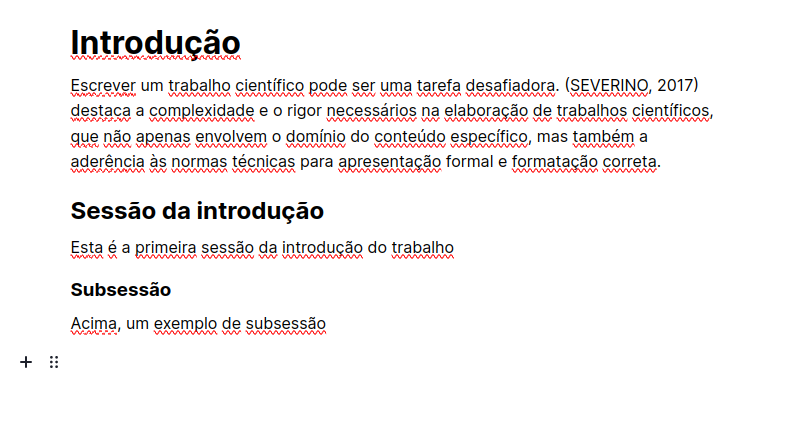
\includegraphics[width=0.9\textwidth]{./images/show-header.png}
    \label{fig:show-header} \\
    \textnormal{\fontsize{10pt}{12pt}Fonte: Autoria própria}
\end{figure}

O nível do título, (Capítulo, sessão e subsessões), é escolhido
a partir do submenu do próprio bloco conforme a
Figura \ref{fig:show-header-1}:

\begin{figure}[H]
    \centering
    \caption{Submenu do Header na interface gráfica}
    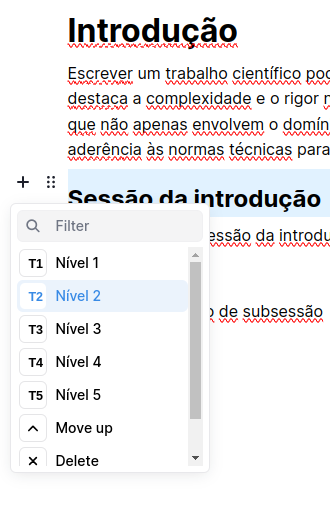
\includegraphics[width=0.4\textwidth]{./images/show-header-1.png}
    \label{fig:show-header-1} \\
    \textnormal{\fontsize{10pt}{12pt}Fonte: Autoria própria}
\end{figure}

\subsubsection{\underline{Paragraph}}

Não há uma construção de um plugin paragraph pois se utiliza
o plugin padrão já pronto fornecido pelo EditorJS.

\subsubsection{\underline{Image}}

O plugin de imagem é um dos mais importantes e complexos do projeto.
É com ele que pode-se trazer ilustrações de imagens para o trabalho escrito,
de forma a enriquecer a monografia, seja ela qual for.

O plugin de imagem possui casos de uso interessantes, como: Trazer imagens
a partir de links ou de arquivos do sistema; Atribuir um título à imagem;
Atribuir uma descrição; Definir a porcentagem de ocupação na folha do documento;
e etc...

\subsubsubsection{O plugin}

Observe na
Figura \ref{fig:class-plugin-image}
a modelagem do plugin de imagem:

\begin{figure}[H]
    \centering
    \caption{Plugin Image}
    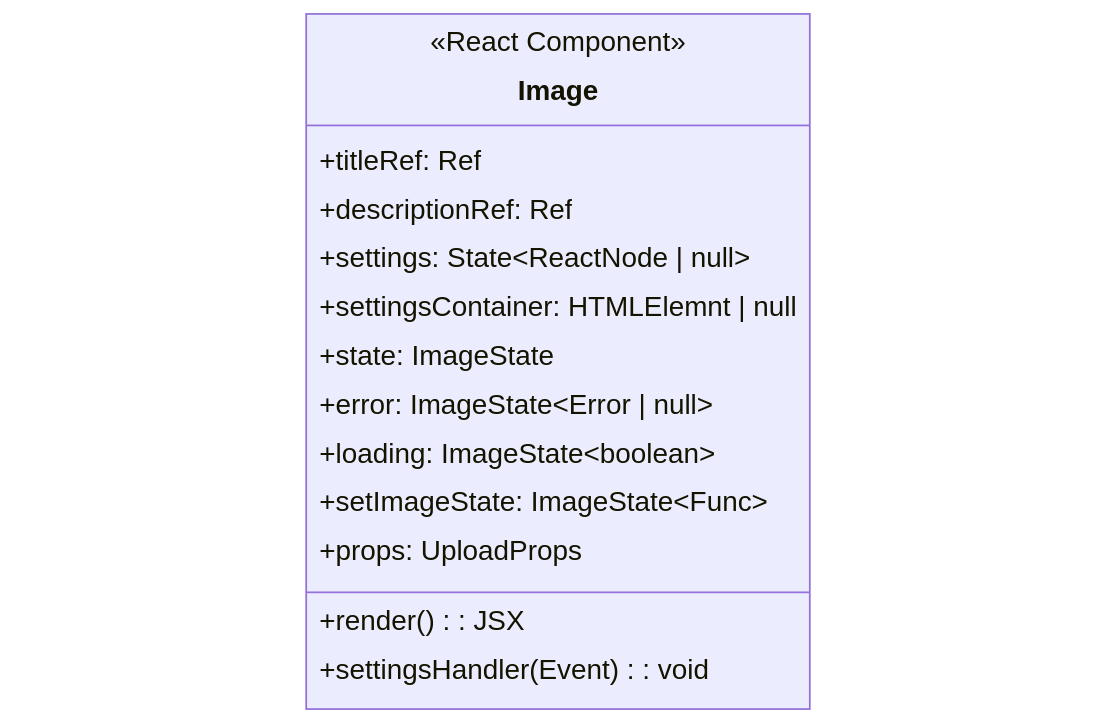
\includegraphics[width=0.8\textwidth]{./images/class-plugin-image.png}
    \label{fig:class-plugin-image} \\
    \textnormal{\fontsize{10pt}{12pt}Fonte: Autoria própria}
\end{figure}

Tem-se primeiramente, as referências a titleRef e descriptionRef, que são
os elementos
\acrshort{html}
que receberão o título e descrição, respectivamente.
Note também que há um estado denominado settings juntamente com settingsContainer,
que guarda um elmento
\acrshort{html}.
Isto se dá devido a uma particularidade do componente Header, pois o mesmo
tem um menu personalizado que se difere do padrão do EditorJs. Este menu é
um componente React que é guardado
no estado settings, que por ventura é renderizado através do portal no elemento
indicado por settingsContainer.

Observe que state; error; loading e setImageState fazem parte de um estado especial
denominado ImageState. Isto se dá devido a complexiade do plugin de imagem, que possui
um hook personalizado em um código separado, de modo a ajudar a gerenciar os casos
de uso do plugin.

O método settingsHandler é o responsável por controlar o estado settings, de modo que
é este quem define quando o menu aparecerá em tela. O controlador do menu é o EditorJs,
que através da chamada de um evento em sua
\acrshort{api}
define quando tal estado será definido.
Desta forma pode-se controlar a renderização de um menu personalizado no EditorJs.

\subsubsubsection{Renderização do componente imagem}

A
Figura \ref{fig:image-component-tree}
demonstra a sub-árvore de renderização do plugin de imagem:

\begin{figure}[H]
    \centering
    \caption{Sub-árvore de renderização do plugin Image}
    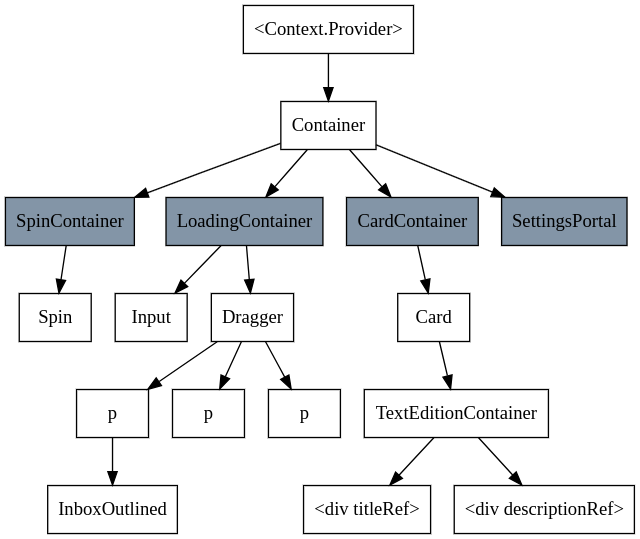
\includegraphics[width=0.8\textwidth]{./images/image-component-tree.png}
    \label{fig:image-component-tree} \\
    \textnormal{\fontsize{10pt}{12pt}Fonte: Autoria própria}
\end{figure}

Observe que há quatro componentes demarcados em azul. Estes componentes
são componentes de renderização condicional, pois o plugin de imagem
altera o seu visual diversas vezes a depender das ações de usuário.

Observe primeiramente o \textit{SpinContainer}. Ele é renderizado sempre que
o estado loading é verdadeiro, ao passo que seus outros três irmãos não.
O SpinContainer nada mais é do que um receptáculo que possui um componente
Spin, que é um indicador animado com papel de mostrar ao usuário que algo está
sendo carregado.

\textit{LoadingContainer} é renderizado quando não há nenhuma imagem atribuída ao componente
e é controlado pelo estado \textit{state}. Possui como filhos um componete Input e Dragger.
O componente Input é onde pode-se colar um link para uma imagem, ao passo que Dragger é
onde se pode arrastar algum arquivo de imagem a partir do Sistema Operacional. O Dragger
também possui três elementos de parágrafos que são textos que orientam o usuário em como
o mesmo pode fazer uso do componente. A
Figura \ref{fig:show-image}
mostra como é a aparência desta parte na interface gráfica.

\textit{CardContainer} é rederizado quando o usuário atribui alguma imagem ao compoente e também
é controlado pelo estado \textit{state}.
Possui um componente Card que vai abrigar a imagem propriamente dita, além também de uma área
textual denominada \textit{TextEditionContainer} onde o usuário pode definir o título e a descrição
da imagem. A
Figura \ref{fig:show-image-image}
demonstra a aparência de um componente imagem com uma imagem atribuída.

Por fim o \textit{SettingsPortal} renderizará uma aparente quebra de árvore no
\acrshort{dom}
do menu do componente. A condição para tal renderização é a chamada do menu
a partir da
\acrshort{api}
do EditorJs. Desta forma, tem-se um componente totalmente integrado ao seu
menu que responde às ações do mesmo e vice versa.
A
Figura \ref{fig:show-image-menu}
mostra a renderização deste menu personalizado.

\subsubsubsection{Aparência do plugin de imagem}

Abaixo é descutida as diversas aparências do plugin de imagem
a depender de seus respectivos estados e ações do usuário.
Inicialmente são renderizadas as instruções para que o usuário possa
atribuir uma imagem ao componente. O desenho de tal tentou ser o mais
simples e objetivo possível, de modo que o usuário não necessite de
nenhum manual para entender o que está acontecendo.

\begin{figure}[H]
    \centering
    \caption{Visual do plugin de imagem}
    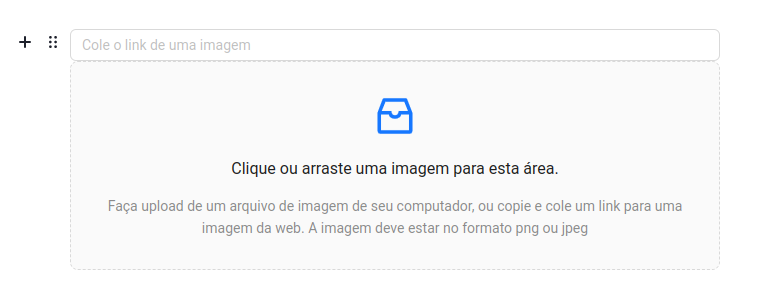
\includegraphics[width=1.0\textwidth]{./images/show-image.png}
    \label{fig:show-image} \\
    \textnormal{\fontsize{10pt}{12pt}Fonte: Autoria própria}
\end{figure}

Quando uma imagem é atribuida, como no caso abaixo, a imagem será exibida
em tela através do editor com um título e uma descrição genérica.
Caso o usuário tenha importando a imagem da internet através de um link, a
descrição padrão automaticamente conterá a referência à sua fonte original.
Note que os campos de título e descrição são editáveis.

\begin{figure}[H]
    \centering
    \caption{Imagem atrelada no plugin}
    
\includegraphics[width=0.9\textwidth]{./images/show-image-image.png}
    \label{fig:show-image-image} \\
    \textnormal{\fontsize{10pt}{12pt}Fonte: Autoria própria}
\end{figure}

O menu de personalização do componente de imagem possui configurações
adicionais. Pode-se alterar a porcentagem de ocupação da imagem no documento,
bem como desatribuir a imagem corrente através do botão limpar. Caso o usuário
desatribuia, o estado retorna para o exibido na
Figura \ref{fig:show-image}.

\begin{figure}[H]
    \centering
    \caption{Sub-menu do plugin de imagem}
    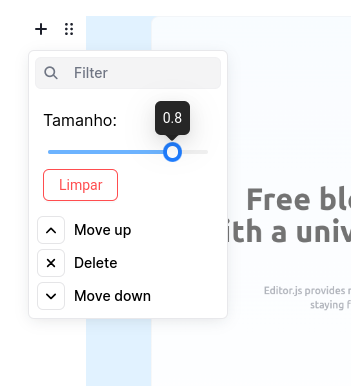
\includegraphics[width=0.6\textwidth]{./images/show-image-menu.png}
    \label{fig:show-image-menu} \\
    \textnormal{\fontsize{10pt}{12pt}Fonte: Autoria própria}
\end{figure}

\subsubsection{\underline{List}}

O plugin List que será utilizado será o padrão fornecido pelo
EditorJS.

\section{Parsing, (parser)}

O processo de Parsing transformará cada bloco provido
pela saída do EditorJs em um trecho de código em
\acrshort{latex}.
Observe na
Figura \ref{fig:parsing-example-header}
e
Figura \ref{fig:parsing-example-paragraph}
os exemplos de parsing aplicados a um objeto de
\textit{Header}\footnote{Do inglês: Cabeçalho. Neste contexto, os headers são os títulos utilizados no documento.
}
e
\textit{Paragraph}\footnote{Do inglês: Parágrafo.
},
respectivamente.

\begin{figure}[H]
    \centering
    \caption{Parsing de um bloco Header}
    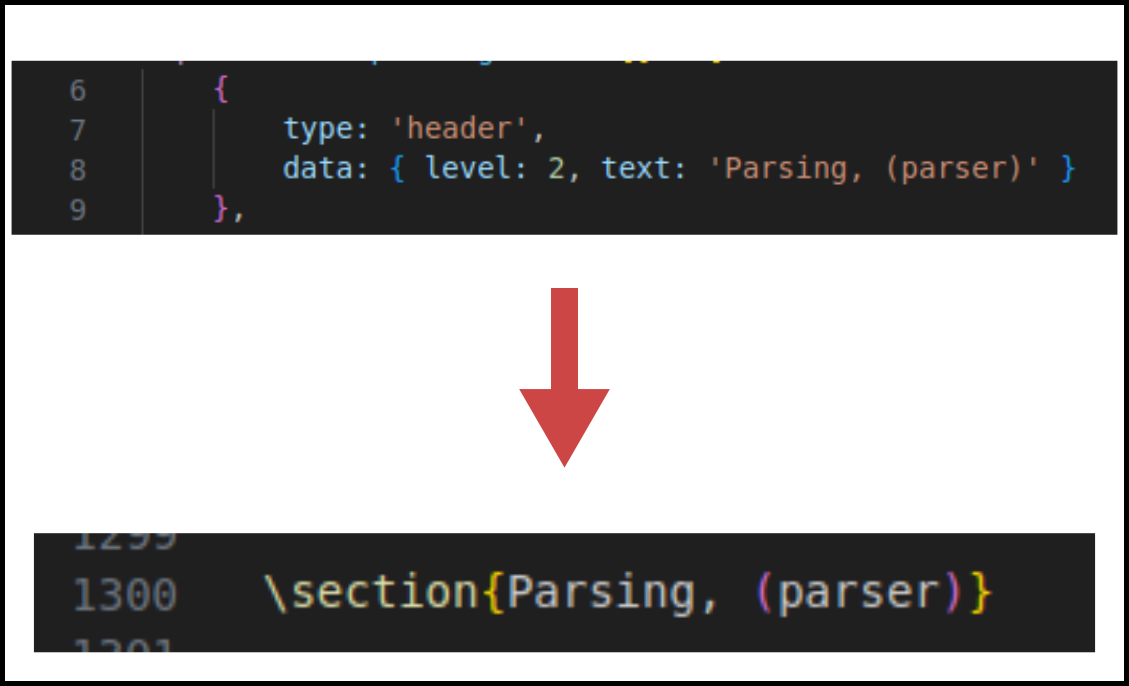
\includegraphics[width=0.8\textwidth]{./images/parsing-example-header.png}
    \label{fig:parsing-example-header} \\
    \textnormal{\fontsize{10pt}{12pt}Fonte: Autoria própria}
\end{figure}

\begin{figure}[H]
    \centering
    \caption{Parsing de um bloco Paragraph}
    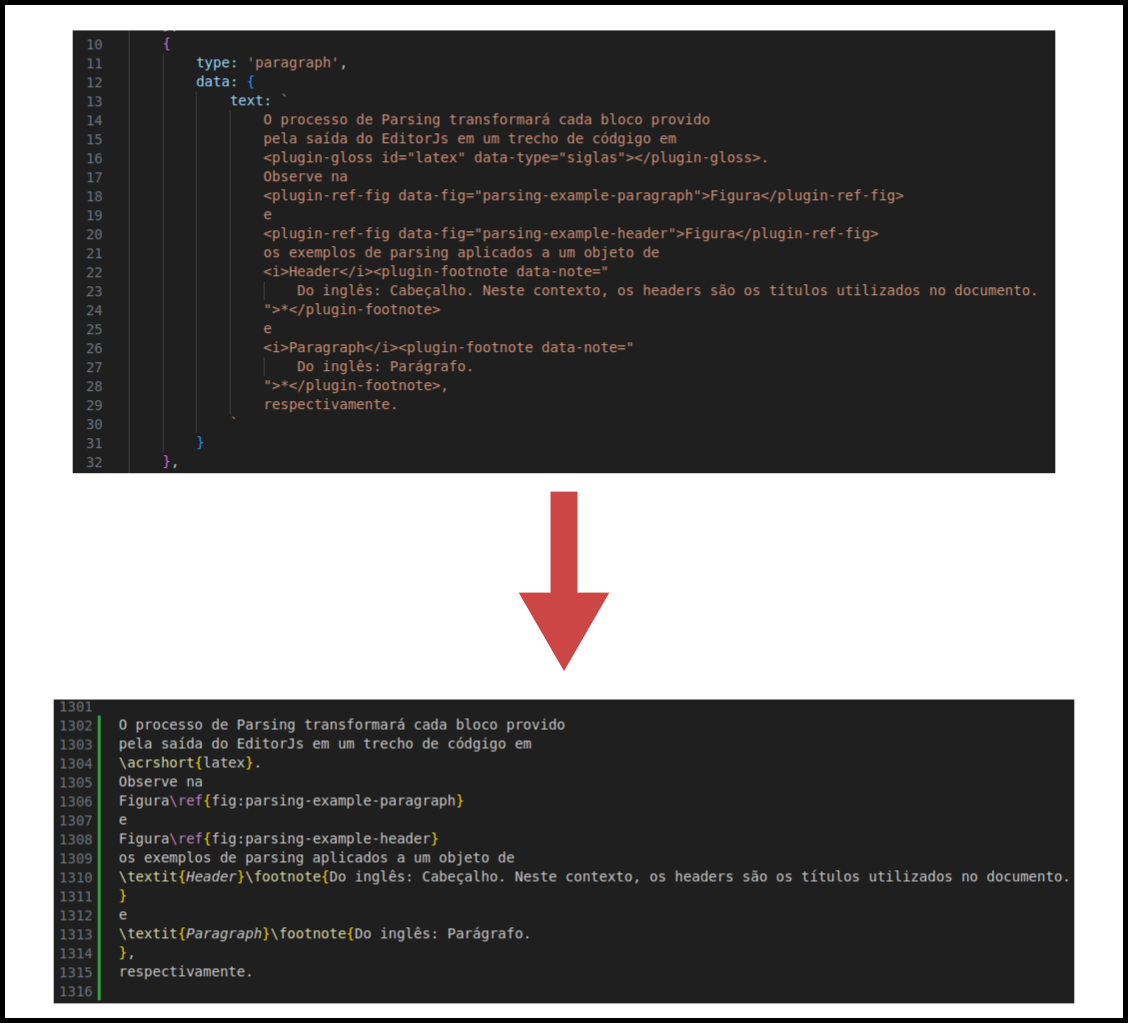
\includegraphics[width=0.8\textwidth]{./images/parsing-example-paragraph.png}
    \label{fig:parsing-example-paragraph} \\
    \textnormal{\fontsize{10pt}{12pt}Fonte: Autoria própria}
\end{figure}

No exemplo do bloco paragraph, é notável o processo de
processamento de
\acrshort{html}
acontecendo. Note que o conteúdo textual do bloco
não é apenas texto simples. Há quatro tags de
marcação personalizadas que se refletem em comandos
especiais
\acrshort{latex}, a saber:

\begin{enumerate}
        
	\item plugin-gloss
	\item plugin-ref-fig
	\item i
	\item plugin-footnote
    
\end{enumerate}

A tabela
Tabela \ref{tbl:plugins-latex-mapping}
mostra o mapeamento destas tags, que são plugins
\textit{in-line}\footnote{Do inglês: Em linha.
}
do EditorJs. As Tags possuem conteúdo e atributo, cada qual se
refletindo a uma particularidade do código
\acrshort{latex}
a depender de sua natureza.

\begin{table}[H]
    \centering
    \caption{Mapeamento de tags em código LaTex}
    \label{tbl:plugins-latex-mapping}
    \renewcommand{\arraystretch}{1.5}
    \begin{tabular}{p{1.9200cm} p{1.9200cm} p{1.9200cm} p{3.2000cm} p{7.0400cm}}
        \hline
        \textbf{Tag} & \textbf{Conteúdo} & \textbf{Atributo} & \textbf{Valor do Atributo} & \textbf{LaTex} \\
        \hline
        plugin-gloss & Não & id & latex & \textbackslash acrshort\{latex\} \\
		plugin-ref-fig & Figura & data-fig & parsing-example-paragraph & \textbackslash ref\{fig:parsing-example-paragraph\} \\
		plugin-ref-fig & Figura & data-fig & parsing-example-header & \textbackslash ref\{fig:parsing-example-header\} \\
		i & Header & Não & Não & \textbackslash textit\{Header\} \\
		plugin-footnote & Não & data-note & <texto da nota> & \textbackslash footnote\{<texto da nota>\} \\
		i & Paragraph & Não & Não & \textbackslash textit\{Paragraph\} \\
		plugin-footnote & Não & data-note & Do inglês: Parágrafo. & \textbackslash footnote\{Do inglês: Parágrafo.\} \\
        \hline
        
    \end{tabular}
\end{table}

\subsection{Visão geral}

O parser da aplicação não depende de nenhuma biblioteca
ou framework de terceiros,
(com excessão do processHTML que utiliza a biblioteca cheerio).
O processo de parsing é feito
apenas utilizando-se de recursos nativos da linguagem
TypeScript, (consequentemente
\acrshort{js}).
A
Figura \ref{fig:estrutura-parser}
mostra a estrutura de pastas do módulo de parse, com três grandes
grupos:

\begin{itemize}
        
	\item process\_steps
	\item plugins
	\item mounting
    
\end{itemize}

O process\_steps diz respeito a funções utilitárias do processamento de texto.
É uma das mais importantes partes pois fornece funções que serão utilizadas a todo
momento em outras partes do parsing. Provê segurança pois nele reside as funções
de escape de caracteres especiais e entre outros.
O plugins fornece o processamento respectivo de cada plugin da aplicação,
bem como o modo em que cada um deverá ser convertido em código
\acrshort{latex}.
O mounting diz respeito a montagens de partes dinâmicas do documento
\acrshort{latex}.

\begin{figure}[H]
    \centering
    \caption{Estrutura de pastas do módulo de parse}
    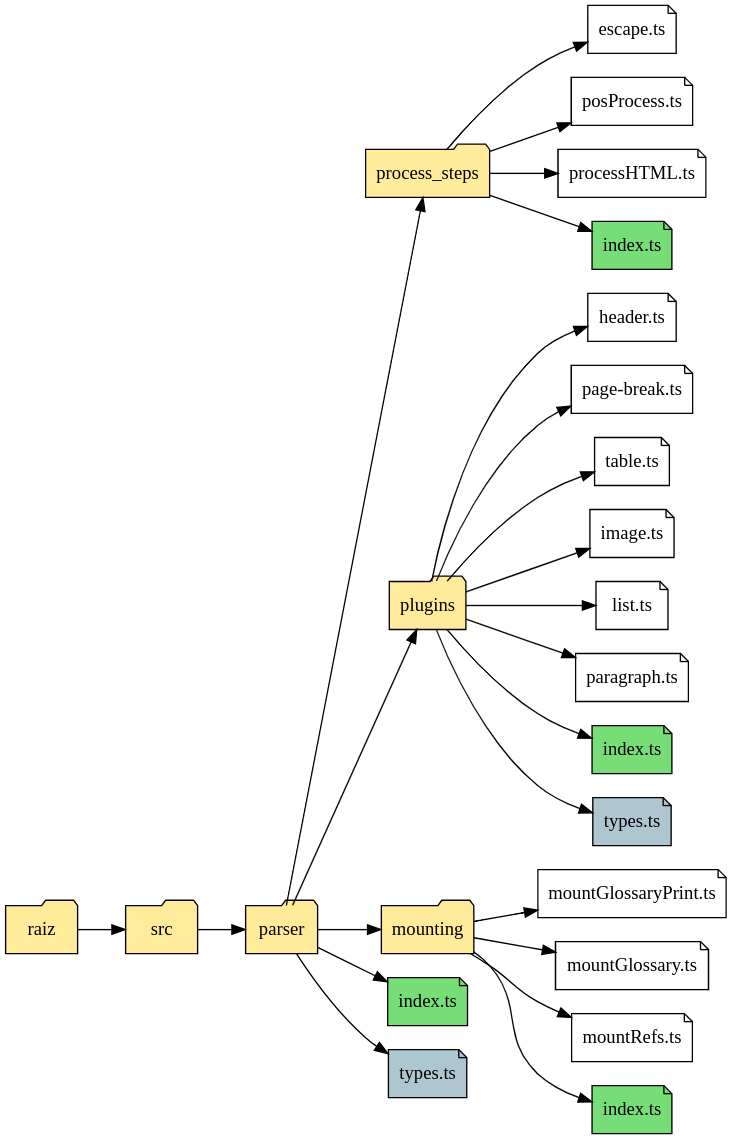
\includegraphics[width=0.8\textwidth]{./images/estrutura-parser.png}
    \label{fig:estrutura-parser} \\
    \textnormal{\fontsize{10pt}{12pt}Fonte: Autoria própria}
\end{figure}

\subsection{Estapas de processamento}

O principal plugin da aplicação a ser processado será o de paragraph.
A informação principal deste plugin é tão somente o texto de marcação
\acrshort{html}. Devido a este fato, este plugin
será o que mais utilizará as funções providadas pelo process\_steps.
A
Figura \ref{fig:fluxo-processamento-texto}
ilustra um ciclo de processamento de texto de marcação:

\begin{figure}[H]
    \centering
    \caption{Um ciclo de processamento de texto}
    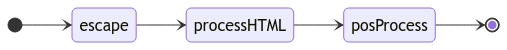
\includegraphics[width=0.9\textwidth]{./images/fluxo-processamento-texto.png}
    \label{fig:fluxo-processamento-texto} \\
    \textnormal{\fontsize{10pt}{12pt}Fonte: Autoria própria}
\end{figure}



\subsubsection{\underline{Escape de caracteres}}

O escape de processamento é a primeira etapa do processamento
de texto. Necessária para evitar o primeiro problema de transformar
o texto de marcação em código
\acrshort{latex},
que é o problema dos caracteres especiais.

O código
\acrshort{latex},
(como dito na fundamentação teórica),
é um código legível tanto para seres humanos
quanto por máquinas. Devido a isto, existem alguns caracteres
especiais de controle que ajudam a definir como
determinado conteúdo aparecerá no documento. Por exemplo:
O caractere \textbackslash~é  um dos mais importantes caracteres do
\acrshort{latex},
pois ele
define uma gama de comandos, como por exemplo o \textbackslash chapter\{\textbf{texto}\},
que define
\textbf{texto}
como sendo um capítulo no documento.
Mas e se o usuário digitar no documento um caractere \textbackslash ?
Quais problemas isso poderá gerar?

Caso o usuário digite um \textbackslash~no documento e este caractere simplesmente seja
transcrito no documento
\acrshort{latex},
gerará uma série de efeitos indesejados, desde
comandos inexistentes como: \textbackslash esse-comando-não-existe,
como o uso acidental de comandos do próprio
\acrshort{latex},
como:
\textbackslash chapter; \textbackslash section ou \textbackslash subsection.
Para evitar isto qualquer ocorrência de
\textbackslash~no texto será substituída por \textbackslash textbackslash, que é um comando
\acrshort{latex}
responsável por imprimir uma \textbackslash~no corpo
do texto.
A
Tabela \ref{tbl:escape-characters}
mostra as ocorrências de todos os caracteres que devem ser substituídos
por algum comando especial no
\acrshort{latex}
que possua o mesmo significado textual:

\begin{table}[H]
    \centering
    \caption{Mapeamento de escape de caracteres para código LaTex}
    \label{tbl:escape-characters}
    \renewcommand{\arraystretch}{1.5}
    \begin{tabular}{p{2.5600cm} p{3.8400cm}}
        \hline
        \textbf{Caractere} & \textbf{Substituição} \\
        \hline
        \textbackslash  & \textbackslash textbackslash  \\
		\# & \textbackslash \# \\
		\$ & \textbackslash \$\$ \\
		\% & \textbackslash \% \\
		\textasciicircum  & \textbackslash textasciicircum  \\
		\& & \textbackslash \& \\
		\_ & \textbackslash \_ \\
		\{ & \textbackslash \{ \\
		\} & \textbackslash \} \\
		{[} & \{{[}\} \\
		{]} & \{{]}\} \\
		\textasciitilde  & \textbackslash textasciitilde  \\
        \hline
        \\\multicolumn{2}{c}{\fontsize{10pt}{12pt}Fonte: Adaptado de: \cite{tutorial-latex}}
    \end{tabular}
\end{table}

Todas as ocorrências destes caracteres devem ser devidadmente
substituídas afim de evitar qualquer problema de interpretação do
compilador
\acrshort{latex}.

\subsubsubsection{Código do escape.ts}

Abaixo tem-se a aplicação do processamento de escape de caracteres
em typescript. a função escapeCharacters recebe uma string na linha 1,
e das linhas 3 a 14 faz uma sucessão de novas atribuições desta nova string.
As atribuições consistem de uma nova string que, através da função replace,
substituem as expressões regulares pela nova string, que seguem de acordo
com a
Tabela \ref{tbl:escape-characters}.
Ao final, na linha 16, a nova string é retornada.

\begin{codeEscape}
export function escapeCharacters(str: string){
    let newStr = str;
    newStr = newStr.replace(/\\/gm, '\\textbackslash ');
    newStr = newStr.replace(/#/gm, '\\#');
    newStr = newStr.replace(/\$/gm, '\\$$');
    newStr = newStr.replace(/%/gm, '\\%');
    newStr = newStr.replace(/\^/gm, '\\textasciicircum ');
    newStr = newStr.replace(/&/gm, '\\&');
    newStr = newStr.replace(/_/gm, '\\_');
    newStr = newStr.replace(/\{/gm, '\\{');
    newStr = newStr.replace(/\}/gm, '\\}');
    newStr = newStr.replace(/\[/gm, '{[}');
    newStr = newStr.replace(/\]/gm, '{]}');
    newStr = newStr.replace(/~/gm, '\\textasciitilde ');

    return newStr;
}
\end{codeEscape}

\subsubsection{\underline{Processamento de HTML}}

O processamento de
\acrshort{html}
é a segunda etapa do processo de parsing. É
nele que os plugins in-line customizados são transformados
em comandos
\acrshort{latex}.
A
Figura \ref{fig:html-processing-example}
inlustra como os plugins de glossário e referência de figuras
se comportam no código
\acrshort{latex}
através dos quadrados coloridos:

\begin{figure}[H]
    \centering
    \caption{Conversão de plugins em código latex}
    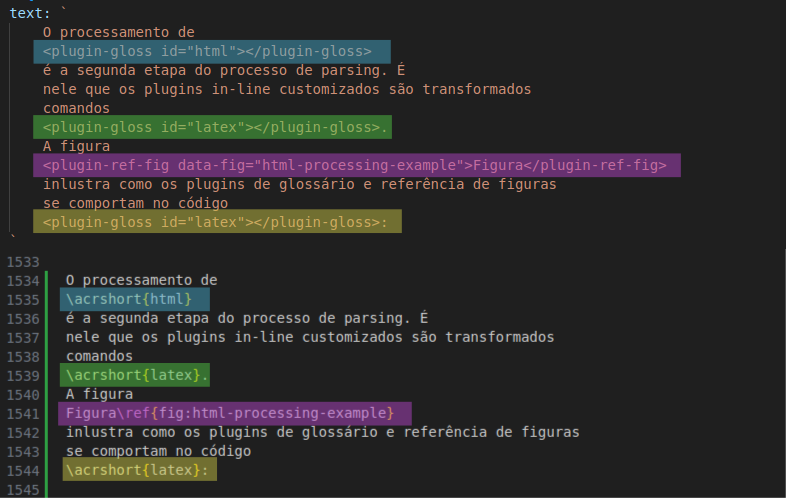
\includegraphics[width=1.0\textwidth]{./images/html-processing-example.png}
    \label{fig:html-processing-example} \\
    \textnormal{\fontsize{10pt}{12pt}Fonte: Autoria própria}
\end{figure}

No caso do plugin-gloss, há também um objeto de glossário que contém todas as definições
de siglas e abreviaturas. Este objeto é transformado e montado em declarações
\acrshort{latex}
para serem usadas ao longo do documento.
Para mais detalhes deste processo, verifique a sessão de montagem

A
Tabela \ref{tbl:plugin-latex-mapping}
mapeia como cada plugin se comportará no código
\acrshort{latex}:

\begin{table}[H]
    \centering
    \caption{Mapeamento de pugins para código latex}
    \label{tbl:plugin-latex-mapping}
    \renewcommand{\arraystretch}{1.5}
    \begin{tabular}{p{3.4496cm} p{3.4496cm} p{6.5856cm}}
        \hline
        \textbf{Tag plugin} & \textbf{Atributo(s)} & \textbf{LaTex} \\
        \hline
        plugin-gloss & id & \textbackslash acrshort\{<id>\} \\
		plugin-ref & id & \textbackslash cite\{<id>\} \\
		plugin-footnote & data-note & \textbackslash footnote\{<data-note>\} \\
		plugin-ref-fig & data-fig & Figura\textbackslash ref\{fig:<data-fig>\} \\
		plugin-ref-table & data-table & Tabela\textbackslash ref\{fig:<data-table>\} \\
		br & Não & \textbackslash \textbackslash  \\
		strong & Não & \textbackslash textbf\{<conteúdo>\} \\
		i & Não & \textbackslash textit\{<conteúdo>\} \\
        \hline
        
    \end{tabular}
\end{table}

Observe que no processamento de
\acrshort{html}
o conteúdo da maioria das tags é irrelevante,
com excessão das tags strong e i.
Isso se dá pois na maioria das vezes a informação
de interesse é guardada nos atributos, ficando
o conteúdo servindo apenas para que se
exiba o plugin de forma confortável no texto que o usuário
está digitando na
\acrshort{ui}.
As tags strong e i, são respectivamente,
o negrito e itálico. São padrões do
\acrshort{html}
e aqui seus conteúdos são aproveitados
para dentro dos comandos equivalentes em
\acrshort{latex}.

\subsubsubsection{Código do processamento HTML}

Para processar os plugins está sendo utilizada a biblioteca cheerio.
A string a ser analisada, recebida na linha 3, passa por uma checagem de
tags presentes. Por exemplo: Observe a linha 5. Sempre que houver
qualquer ocorrência de plugin-ref, esta é substituída através do
comando replaceWith pelo texto:
\textbackslash cite\{\$\{\$(node).attr('id')\}\}.
Observe que a parte \$(node).attr('id')
é o que recupera o atributo "id"~  da tag.

\begin{processHTML}
import * as cheerio from 'cheerio';

export function processHTML(text: string): string{
    const $ = cheerio.load(text);
    $('plugin-ref').replaceWith((_, node) => {
        return `\\cite{${$(node).attr('id')}}`;
    }); [...]
\end{processHTML}

Por fim, na linha 40 é retornado o resultado do processamento
em HTML. Note que ele é recuperado a partir do nó body do documento
virtual, e então, a função text() é chamada para recuperar a
representação textual do que foi processado.

\begin{processHTML2}
[...]
    return $('body').text();
}
\end{processHTML2}

O código completo do processHTML.ts juntamente com
todos os plugins pode ser encontrado no repositório do projeto.

\subsubsection{\underline{Pós processamento}}

Após feito o processo de escape e processamento de HTML, ainda podem
sobrar alguns caracteres remanescentes problemáticos à correta
interpretação do código
\acrshort{latex}.
Por exemplo: Os caracteres < e > são escapados no
\acrshort{html}
como as entidades lt e gt, respectivamente. Eles por sua vez,
ao passar pelo escape de caracteres, possuem o caractere
\& escapado como \textbackslash \&. Seu código final acaba resultando em
\textbackslash < e \textbackslash >, que tem de novamente ser convertido em
< e >.
Observe o código abaixo:

\begin{posProcess1}
export function posProcess(str: string): string{
    let new_str = str.replace(/\\</gm, '<');
    new_str = new_str.replace(/\\>/gm, '>');
    new_str = new_str.replace(/\\"/gm, '"');
    new_str = new_str.replace(
        /"(?!\w|\}|\)|\\|~|\.|,|\{|\(|\[)/gm,
        '"~'
    );
    new_str = new_str.replace(
        /(\\textbackslash)((\s?\n)|(\s{2,}))/gm,
        '$1~'
    );
    return new_str;
}
\end{posProcess1}

\subsection{Plugins}

O parsing dos plugins é algo essencial na montagem
do documento ao qual estar-se a escrever. São os plugins
que formam cada pequena unidade de bloco que comporá
um documento que muitas vezes se tornará gigantesco.

\subsubsection{\underline{Tipagem}}

\begin{figure}[H]
    \centering
    \caption{Caminho da pasta types dos plugins no parser}
    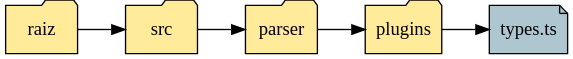
\includegraphics[width=0.8\textwidth]{./images/src-parser-plugins-types.png}
    \label{fig:src-parser-plugins-types} \\
    \textnormal{\fontsize{10pt}{12pt}Fonte: Autoria própria}
\end{figure}

O arquivo de tipagem é onde é concentrada todas as anotações
de tipo de cada bloco. O documento todo é um array de objetos,
no qual cada um desses objetos corresponde a um bloco
do documento. É através de cada tipo de bloco que pode-se por exemplo,
discriminar qual tipo de bloco está sendo tratado no momento do processamento.
Observe por exemplo a anotação de tipo do ParagraphBlock:

\begin{ParagraphBlockCode}
[...]
export interface ParagraphBlock {
    type: 'paragraph'
    id: string
    data: {
        text: string
    }
}
[...]
\end{ParagraphBlockCode}

Todo bloco é composto basicamente por estas três propriedades:
type; id e data. Sendo que a propriedade data variará sua
forma a depender do bloco que está sendo definido. Este código
nunca é executado ou incluido na versão de execução final em
\acrshort{js},
(por se tratar de uma anotação de tipo). Mas é de extrema
utilidade quando se trata de guiar o desenvolvedor na hora
de instanciar um objeto do tipo que é definido pelo
interface\footnote{Neste contexto, está-se utilizando o termo interface em seu original
    inglês, conforme a documentação do TypeScript. Devido a este fato,
    interface (não confundir com interface de usuário) será tratado
    com pronome masculino.
}
ParagraphBlock.

Observe como o interface do HeaderBlock se diferencia
do ParagraphBlock em sua anotação de tipo:

\begin{HeaderBlockCode}
[...]
export interface HeaderBlock {
    type: 'header'
    id: string
    data: {
        level: 1 | 2 | 3 | 4 | 5
        text: string
    }
}
[...]
\end{HeaderBlockCode}

No HeaderBlock, a propriedade data é composta por outras duas propriedades: text e level.
Ao refletir sobre isso, percebe-se que essas duas propriedades são essenciais para definir
o que é um título em um documento. O level (nível) indica o nível hierárquico do título,
enquanto o text (texto) representa o conteúdo exibido como título. Perceba que há uma
limitação na definição do nível do título, com valores variando apenas de 1 a 5.
Cada um desses valores corresponde respectivamente às sessões: primária, secundária, terciária, quaternária e quinária.

Observe na
            Tabela \ref{tbl:header-level-latex}
            a relação do level do título com o código
            \acrshort{latex}
            correspondente:

\begin{table}[H]
    \centering
    \caption{Relação do level do título com o código latex}
    \label{tbl:header-level-latex}
    \renewcommand{\arraystretch}{1.5}
    \begin{tabular}{p{1.0320cm} p{5.8480cm}}
        \hline
        \textbf{Level} & \textbf{Código LaTex} \\
        \hline
        1 & \textbackslash chapter\{<conteúdo>\} \\
		2 & \textbackslash section\{<conteúdo>\} \\
		3 & \textbackslash subsection\{<conteúdo>\} \\
		4 & \textbackslash subsubsection\{<conteúdo>\} \\
		5 & \textbackslash subsubsubsection\{<conteúdo>\} \\
        \hline
        
    \end{tabular}
\end{table}

\subsubsection{\underline{Paragraph, (parágrafo)}}

O bloco de parágrafo parece de longe um dos blocos mais simples de todos.
Ele simplesmente retorna o texto do bloco recebido, fazendo-o passar
pelas etapas de processamento conforme já descrito na
Figura \ref{fig:fluxo-processamento-texto}.
Observe na linha 7 como o parâmetro block é anotado com o tipo ParagraphBlock.
É neste caso que entra a utilidade do TypeScript. Pois além de prevenir erros
não deixando que se passe um bloco incorreto para ser processado por essa função,
tem-se a condição de saber exatamente o que tem dentro da propriedade
data na linha 11. Neste caso, apenas passa-se o texto para o processamento.

\begin{getParagraphCode}
import { escapeCharacters } from '@/parser/process_steps/escape';
import { processHTML } from '@/parser/process_steps/processHTML';
import { ParagraphBlock } from '@/parser/types';
import { posProcess } from '@/parser/process_steps/posProcess';


export function getParagraph(block: ParagraphBlock){
    return posProcess(
        processHTML(
            escapeCharacters(
                block.data.text
            )
        )
    );
}
\end{getParagraphCode}

\subsubsection{\underline{Header, (cabeçalhos)}}

O parse do bloco de Header já distoa-se um pouco do bloco de paragraph.
Aqui é notável a aplicação do exposto na
Tabela \ref{tbl:header-level-latex}
onde o cada level se traduz em um comando diferente no latex. Através da
clausula switch, o level é testado afim de retornar as particularidades
de cada tipo de título. Observe que o level 4, implementado na linha 13,
possui um comando a mais de \textbackslash underline para que o título
apareça como sublinhado. Este comando a mais foi implementado
para atender as particularidades exidas pelo documento da
\acrshort{pucgo}
em:
\cite{pucgo}.

\begin{getHeaderCode}
import { escapeCharacters } from '@/parser/process_steps/escape';
import { HeaderBlock } from '@/parser/types';

export function getHeader(block: HeaderBlock){
    switch(block.data.level){
        case 1:
            return `\\chapter{${escapeCharacters(block.data.text)}}`
        case 2:
            return `\\section{${escapeCharacters(block.data.text)}}`
        case 3:
            return `\\subsection{${escapeCharacters(block.data.text)}}`
        case 4:
            return `\\subsubsection{\\underline{${
                escapeCharacters(block.data.text)
            }}}`
        case 5:
            return `\\subsubsubsection{${
                escapeCharacters(block.data.text)
            }}`
    }
}
\end{getHeaderCode}

\subsubsection{\underline{Image, (imagens)}}

O parse do plugin de imagem é um dos mais complexos em termos de comandos
\acrshort{latex}. Ele retorna toda uma estrutura
de modo que o compilador de documentos
\acrshort{latex}
possa renderizar a imagem corretamente e seja capaz
de referenciá-la ao longo do texto.

Nas linhas 8 a 12 tem-se a desconstrução das propriedades da
imagem que estão presentes na propriedade data do bloco.
Estas propriades são:
\acrshort{uuid}\footnote{\acrshort{UUID},
    \textit{Universally Unique Identifier}
    (Identificador Universalmente Único).
};
title; width; description e fileType.

\begin{getImageCode1}
import { escapeCharacters } from '@/parser/process_steps/escape';
import { posProcess } from '@/parser/process_steps/posProcess';
import { processHTML } from '@/parser/process_steps/processHTML';
import { ImageBlock } from '@/parser/types';

export function getImage(block: ImageBlock){
    const {
        uuid,
        title,
        width,
        description,
        fileType,
    } = block.data;
[...]
\end{getImageCode1}

Na linha 20 tem-se a inclusão do título da imagem. Note que
o título somente precisa passar pelo processo de escape de caracteres,
uma vez que no mesmo não haverá plugins no corpo do texto.
Nas linhas 25 à 33 há a inclusão da descrição da imagem.
Note que diferente do título, a descrição passa por todo o
ciclo de processamento, pois na descrição o usuário pode incluir
referências e outras coisas que resultam na presença de tags
de plugin no corpo do texto.

As linhas 21 a 23 tratam do tamanho que a imagem vai ocupar
na tela, bem como a referência ao arquivo de imagem que
será renderizado. As propriedades width,
\acrshort{uuid},
e fileType
são utilizadas neste processo. Cada imagem é guardada na
pasta interna images com o nome do
\acrshort{uuid}
que o software
define, bem como sua extensão de arquivo.

A linha 24 utiliza o
\acrshort{uuid}
para definir a label da imagem.
Desta forma, a imagem a que se trata o bloco torna-se
referenciável no texto do documento.

\begin{getImageCode2}
[...]


// H Prevents figure to be placed incorrectly
return `
    \\begin{figure}[H]
        \\centering
        \\caption{${escapeCharacters(title)}}
        \\includegraphics[width=${
            width.toFixed(1)
        }\\textwidth]{./images/${uuid}.${fileType}}
        \\label{fig:${uuid}} \\\\
        \\textnormal{\\fontsize{10pt}{12pt}${
            posProcess(
                processHTML(
                    escapeCharacters(
                        description
                    )
                )
            )
        }}
    \\end{figure}
`.trim().replace(/^\s{8}/gm, '');
}
\end{getImageCode2}

\subsubsection{\underline{List, (listas)}}

Existem dois tipos de lista, as enumeradas e as não enumeradas, respectivamente
enumerate e itemize no código
\acrshort{latex}.
A linha 9 utiliza a propriedade type para definir qual tipo de lista será utilizada.
Por fim, a lista é composta de uma iteração sobre as strings do array presente
na propriedade list. Este array, após ajustado com a função map, é transformado
em uma string unindo seus itens por uma quebra de linha com o auxílio da
função join na linha 11. Observe também o processamento textual presente na
linha 11. Isso se dá pela liberdade do usuário em utilizar plugins nos
campos de lista.

\begin{getListCode1}
import { escapeCharacters } from "@/parser/process_steps/escape";
import { processHTML } from "@/parser/process_steps/processHTML";
import { ListBlock } from "@/parser/types";
import { posProcess } from "@/parser/process_steps";

export function getList(list: ListBlock){
    const { data: { type, list: __list } } = list;
    return `
    \r\\begin{${ type === 'bullet' ? 'itemize' : 'enumerate' }}
        ${__list.map(el => `\r\t\\item ${
            posProcess(processHTML(escapeCharacters(el))) }`).join('')
        }
    \r\\end{${ type === 'bullet' ? 'itemize' : 'enumerate' }}
    `.trim()
}
\end{getListCode1}

\subsubsection{\underline{Page Break, (quebra de página)}}

O bloco de PageBreak é o bloco de parser mais simples de todos.
Embora receba como parâmetro um bloco do tipo PageBreakBlock,
nem uso do mesmo é feito.
O PageBreak apenas retorna um comando em
\acrshort{latex}
que limpa a página e faz com que o conteúdo após o mesmo
seja escrito na próxima página.

\begin{getPageBreak1}
import { PageBreakBlock } from '@/parser/types';

export function pageBreak(block: PageBreakBlock){
    return '\\clearpage';
}
\end{getPageBreak1}

\subsection{Montagem}

O processo de montagem é o processo no qual algumas partes do código
\acrshort{latex}
são montadas separadamente para fins de organização.
Após montadas, cada uma destas partes são incluídas no código principal
através do comando \textbackslash input.

\subsubsection{\underline{Glossário}}

Cada item de glossário, seja ele uma abreviação ou sigla,
deve ser definido no documento antes que se possa fazer uso do mesmo.
Observe abaixo o exemplo de uma definição de sigla em
\acrshort{latex}:

\begin{Codedc0ef1ab89ac477c95e4876bf47337cf}
\newacronym[type=sigla]{abnt}{ABNT}{
    Associação Brasileira de Normas Técnicas
}
\end{Codedc0ef1ab89ac477c95e4876bf47337cf}

Além de montados, cada clossário deve ser exibido com o comando
\textbackslash printglossary. Veja o código abaixo:

\begin{Code3285f493bfef4e12aff838e3f042c3f5}
\printglossary[type=sigla,title=LISTA DE SIGLAS]
\clearpage

\printglossary[type=abreviacao,title=LISTA DE ABREVIATURAS]
\clearpage
\end{Code3285f493bfef4e12aff838e3f042c3f5}

Isto garante que os devidos glossários sejam exibidos com
folga de uma página, com seus respectivos títulos.

A função mountGlossary exportada em mountGlossary.ts
contém sua implementação, que faz todo o processamento dos
items de glossário a partir de um GlossaryObjectType:

\begin{Codedf3f2b4d01cb459594a489dc923437ff}
[...]
export function mountGlossary(glossary: GlossaryObjectType){
    const header = `
        \\newglossary*{abreviacao}{Lista de abreviaturas}
        \\newglossary*{sigla}{Lista de siglas}
        \\newglossary*{simbolo}{Lista de símbolos}
    `.trim().replace(/^\s{8}/gm, '');

    const gloss_arr = Object.keys(glossary).map(
        key => ({ ...glossary[key], key })
    );

    const acronyms = gloss_arr
        .filter(({ type }) => type === 'sigla')
        .sort(({ label: a }, { label: b }) => a.localeCompare(b))
        .map(({ short, label, type, key }) => {
            return `\\newacronym[type=${type}]{${key}}{${
                escapeCharacters(short)
            }}{${
                escapeCharacters(label)
            }}`
        })
        .join('\n');
\end{Codedf3f2b4d01cb459594a489dc923437ff}

Note que todos os objetos de glossário vem misturados
no parâmetro glossary da função.
Para montar as siglas da linha 15,
por exemplo, é feita uma filtragem no tipo de glossário, uma
ordenação através da função sort, e por fim, a conversão em código
\acrshort{latex}
através da função map na linha 18. Por fim, o array de siglas
é unido através do caractere de quebra de linha por meio da função
join em 25. O mesmo processo acontece com a lista de abreviações
e de termos.

Por fim, basta unir tudo em uma string conforme mostrado na linha
65 e 66 abaixo. As linhas 68 e 69 foram uma tentativa de customizar o estilo
do glossário e seu título. Por hora, esta parte está omitida do trabalho.
A linha 67 adiciona o comando \textbackslash makeglossaries, que diz ao
\acrshort{latex}
para montar o glossário.

\begin{Code8328ef9f627f4fa589e576435ea8ad90}
[...]
    let str = `${header}\n\n${acronyms}\n`;
    str = str.concat(`${abbreviations}\n${symbols}\n\n`);
    str = str.concat(`\\makeglossaries`);
    // str = str.concat('\n\n').concat(custom_style);
    // str = str.concat('\n\n').concat(custom_title);


    return str;
}
\end{Code8328ef9f627f4fa589e576435ea8ad90}

Após todo o processamento seu resultado é guardado em um arquivo
denominado makeGlossaries.tex a ser importado posteriormente
pelo código fonte contruído no processo de Parsing.

\subsubsection{\underline{Referências}}

A parte de referênciação é uma das automações mais úteis do projeto, pois
adiciona referências cruzadas ao projeto facilmente navegável na versão
digital do mesmo.

Observe a função mountRefs exportada a partir do arquivo mountRefs.ts:

\begin{Codeb4ac89d0dbbd4880af6dbd2386fc6ea5}
import { RefsObjectType } from '@/parser/types';

export function mountRefs(refs: RefsObjectType){
    return Object.keys(refs).map(key => {
        const ref  = refs[key];
        const { type, ...restRefs } = ref;
        if(type){
            return `
                @${type}{${key},
                    ${(() => {
                        return Object.keys(restRefs).map(ref_key => {
                            switch(type){
                                case 'misc':
                                case 'book':
                                case 'article':
                                    // @ts-ignore
                                    const value = restRefs[ref_key];
                                    if(ref_key === 'author')
                                        return `${ref_key}={${
                                            (value as string[])
                                                .join(' and ')
                                    }}`
                                    else if(ref_key === 'edition')
                                        return `${ref_key}={${
                                            (value as number)
                                                .toString()
                                                .concat('st')
                                    }}`
                                    else
                                        return `${ref_key}={${value}}`
                            }
                        }).join(',\n    ')
                    })()}
                }
            `.trim().replace(/^\s{16}/gm, '');
        }

        return '';
    }).join('\n\n');
}
\end{Codeb4ac89d0dbbd4880af6dbd2386fc6ea5}

\chapter{Considerações finais}

Este instrumento visou durante seu processo de
elaboração o desenvolvimento da plataforma de modo
que a mesma seja uma ferramenta útil e de
facil compreensão para o mais diverso público.
Desta forma, o usuário da ferramenta precisa se preocupar
apenas com seu conteúdo defendido, de modo que a forma de
sua apresentação é um encargo da ferramenta.

Esta concepção inicial constitui-se numa proposta de mudança 
de paradigma na forma e no fluxo com que se escreve um trabalho
acadêmico, fornecendo uma alternativa mais amigável às formas
tradicionais de escrita utilizando-se o \textit{Microsoft Word},
\textit{Libre Office} ou o próprio
\acrshort{latex}
em sua forma pura.

\section{O que foi desenvolvido}

Foi desenvolvido um programa aplicativo, no modelo cliente-servidor,
que serve um sistema
\acrshort{web}
para o usuário final. O sistema consiste em um rico editor de texto
baseado em blocos em que, através de plugins, monta-se todo um complexo
trabalho de monografia constituído de pequenos blocos simples.

O processo de parsing se encontra totalmente funcional para todos os seguintes blocos:

\begin{itemize}
        
	\item Code, (código)
	\item DirectCite, (citação direta)
	\item Header, (cabeçalhos, títulos)
	\item Image, (imagens)
	\item List, (listas)
	\item PageBreak, (quebra de página)
	\item Paragraph, (parágrafo)
	\item Table, (tabelas)
    
\end{itemize}

Deste modo, qualquer bloco saída do editor já é devidamente transpilado para seu equivalente
código
\acrshort{latex}
e consequentemente compilado no
\acrshort{pdf} final.

Em se tratando da interface do editor com o usuário, nem todos os blocos plugins foram desenvolvidos
conforme a proposta inicial deste instrumento, (vide "O que deu errado"~ e "Trabalhos futuros").
Os seguintes plugins encontram funcionais no editor:

\begin{itemize}
        
	\item Paragraph, (parágrafo)
	\item Header, (cabeçalho)
	\item Image, (Imagem)
    
\end{itemize}

Este trabalho não foi desenvolvido utilizando-se o aplicativo em sua interface gráfica, mas utilizou todos os recursos providos pelo processo de parsing. O código de saída do editor foi escrito manualmente e em seguida compilado. O processo de compilação pode ser repetido rodando o comando abaixo a partir da pasta raiz do projeto no GitHub:

\begin{Code73c00f5bd5584eb4b4a1f1de6b70549c}
yarn tex-make
\end{Code73c00f5bd5584eb4b4a1f1de6b70549c}

\section{O que deu errado}

Devido a duração do processo de pesquisa e do prazo determinado para a finalização deste instrumento,
alguns plugins não foram desenvolvidos ou foram desenvolvidos parcialmente. Os plugins in-line, que consistem
na atribuição de glossários e referências bibliográficas, não foram desenvolvidos para a interface gráfica,
porém possuem seus equivalentes em termos de parsing.

\section{Performance}

Todo este trabalho foi desenvolvido utilizando-se do processo de parsing desenvolvido pelo mesmo, ao passo que
paralelamente foi desenvolvida a interface.
O código
\acrshort{latex}
resultante gerou um arquivo texto de aproximadamente 176kb, que foi compilado sem demais problemas
e com um tempo de menos de 60 segundos. Além também de mais de 2000kb em imagens.

\section{Trabalhos futuros}

Há muitas coisas novas que podem ser implementadas e desenvolvidas a partir da concepção inicial deste trabalho.
Plugins novos podem ser desenvolvidos e ajustes de interface e melhorias de experiência de usuário podem
ser implementados.

\subsection{Plugins inline}

Os plugin inline são de grande importância para uma boa experiência de usuário
e escrita prazerosa. Através deles podem-se atribuir glossários, referências cruzadas
a tabelas e figuras, e referências bibliográficas. Seus respectivos códigos de parsing
encontram-se integrados ao projeto, porém seus equivalentes em termos de interface
e experiência de usuário ainda não foram desenvolvidos.

\subsection{Tabelas}

As tabelas são plugins úteis na exbição e organização de determinados tipos de informação.
Seu parsing encontra-se no projeto poŕém ainda não há o equivalente plugin integrado ao editor.

\subsection{Matemática}

O
\acrshort{latex}
é bastante versátil em termos de equações matemáticas. Neste sentido, pode-se
desenvolver um plugin em que o usuário possa digitar as equações na sintaxe
matemática do
\acrshort{latex}
ou ainda uma interface low code em que o mesmo possa
escrevê-las clicando em ícones na tela.

\subsection{Gráficos e diagramas}

Uma grande utilidade poderia ser a integração com bibliotecas e frameworks
como Mermaid e Graphviz. Estas bibliotecas são de facil compreensão e muito
úteis na hora de criar qualquer tipo de gráfico ou diagrama.

\section{Finalização}

Levando-se em consideração todas as funcionalidades desenvolvidas, (principalmente no que diz
respeito à questão de parsing), o sistema funcionou de forma coerente trazendo bons resultados,
se apresentando como uma solução sub-ótima, levando-se em consideração a concepção inicial.